\documentclass[a4paper,10pt,headings=normal,bibliography=totoc]{scrartcl}

\usepackage{scrhack}  % Fix a LaTeX warning

%%%%%%%%%%%%%%%%%%%%%%%%%%%%%%%%%%%%%%%%%%%%%%%%%%%%%%%%%%%%%%%%%%%%%%%%%%%%%%%
\usepackage[utf8x]{inputenc}
\usepackage{amsmath}
\usepackage{amssymb}
\usepackage{amsthm}
\usepackage{bm}
\usepackage{colonequals}
\usepackage{overpic}
\usepackage{url}
\usepackage{xspace}
\usepackage[square,numbers,sort]{natbib}

\usepackage[colorinlistoftodos]{todonotes}
%\usepackage[colorinlistoftodos,disable]{todonotes}
\usepackage{environ}
\usepackage{enumitem}
\usepackage{listings}
\usepackage{float}


\usepackage{tikz}
\usetikzlibrary{arrows}
\tikzset{
    treenode/.style = {
        align=center,
        inner sep=0pt,
        text centered,
        font=\sffamily,
        rectangle,
        rounded corners=3mm,
        draw=black,
        minimum width=2em,
        minimum height=2em,
        inner sep=1mm,
        outer sep=0mm
    },
    basisnode/.style = {
        treenode,
        minimum width=9mm,
    }
}


%%%%%%%%%%%%%%%%%%%%%%%%%%%%%%%%%%%%%%%%%%%%%%%%%%%%%%%%%%%%%%%%%%%%%%%%%%%%%%%
%%%%%%%%%%%   hyperref should be loaded late to avoid incompatibilities
\usepackage[pdftitle={Function space bases in the dune-functions module},
            pdfauthor={Christian Engwer, Carsten Gräser, Steffen Müthing, and Oliver Sander}]
             {hyperref}

\usepackage{attachfile2}
\usepackage{fancyvrb}

%%%%%%%%%%%%%%%%%%%%%%%%%%%%%%%%%%%%%%%%%%%%%%%%%%%%%%%%%%%%%%%%%%%%%%%%%%%%%%%
%%%%%%%%%%%%     Settings for the listings package
\lstset{language={c++},
         basicstyle=\ttfamily\small,
         keepspaces=true,
%         commentstyle=\textit,
         commentstyle=\rmfamily\textit,
%         columns=fixed,
         columns=flexible,
         escapeinside={/*@}{@*/},
         moredelim=**[is][\color{blue}]{@@}{@@},
        }

% How to include ranges of an external source code file
\lstset{rangeprefix=//\ \{\ ,% curly left brace plus space, all in a C++-style comment
        rangesuffix=\ \},% space plus curly right brace
        numberstyle=\footnotesize,  % font size for numbers
        includerangemarker=false}  % Do not show the range markers


\lstdefinestyle{Example}{}
\lstdefinestyle{Interface}{backgroundcolor=\color{lightblue},frame=single}

\newcommand{\cpp}[1]{\lstinline[basicstyle=\ttfamily]!#1!}



\newtheorem{definition}{Definition}

%%%%%%%%%%%%%%    Define a 'shellenv' environment for shell output
\usepackage{fancyvrb}

\DefineVerbatimEnvironment%
 {shellenv}{Verbatim}
 {}


%%%%%%%%%%%%%%%%%%%%%%%%%%%%%%%%%%%%%%%%%%%%%%%%%%%%%%%%%%%%%%%%%%%%%%%%%%%%%%%

\newcommand{\R}{\mathbb{R}}
\newcommand{\N}{\mathbb{N}}
\newcommand{\abs}[1]{{\lvert#1\rvert}}
\newcommand{\norm}[1]{\lVert#1\rVert}
\newcommand{\op}[1]{\operatorname{#1}}
\newcommand{\st}{\; : \;}
\renewcommand{\div}{\operatorname{div}}
\DeclareMathOperator{\trace}{tr}

\newcommand{\dune}{\textsc{Dune}\xspace}
\newcommand{\program}[1]{\textsc{#1}\xspace}



% For typesetting Dune module names
\newcommand{\dunemodule}[1]{\texttt{#1}}
% For typesetting file names
\newcommand{\file}[1]{\texttt{#1}}

\definecolor{lightblue}{HTML}{55AAFF}

\newcommand{\todosander}[1]{\todo[inline,color=orange,author=OS]{#1}}
\newcommand{\todograeser}[1]{\todo[inline,color=lightblue,author=CG]{#1}}

%%  All graphics files must be in this subdirectory
\graphicspath{{gfx/}}

%%%%%%%%%%%%%%%%%%%%%%%%%%%%%%%%%%%%%%%%%%%%%%%%%%%%%%%%%%%%%%%%%%%%%%%%%%%%%%%%%%%%%%%%%%%%%%%%%%%%%
%%%%%%%%%%%%%%%%%%%%%%%%%%%%%%%%%%%%%%%%%%%%%%%%%%%%%%%%%%%%%%%%%%%%%%%%%%%%%%%%%%%%%%%%%%%%%%%%%%%%%
%%%%%%%%%%%%%%%%%%%%%%%%%%%%%%%%%%%%%%%%%%%%%%%%%%%%%%%%%%%%%%%%%%%%%%%%%%%%%%%%%%%%%%%%%%%%%%%%%%%%%

\title{Function space bases in the dune-functions module}
\author{Christian Engwer, Carsten Gräser, Steffen Müthing, and Oliver Sander}
%\date{}

\begin{document}

\maketitle

\begin{abstract}
 \dunemodule{dune-functions} is a \dune module that provides interfaces for functions and function space bases.
 It forms one abstraction level above grids, shape functions, and linear algebra, and provides infrastructure
 for full discretization frameworks like \dunemodule{dune-pdelab} and \dunemodule{dune-fem}.
 This document describes the function space bases provided by \dunemodule{dune-functions}.  These are
 based on an abstract description of bases for external sum spaces as trees of simpler bases.
 From this description, orderings of degrees of freedom and their numbering by multi-indices can be
 derived in a natural way. We describe the abstract concepts, document the programmer interface,
 and give a complete example program that solves the stationary Stokes equation using Taylor--Hood elements.
\end{abstract}

\section*{Introduction}

The core modules of the \dune software system have always focused on low-level infrastructure for
implementations of simulation algorithms for partial differential equations.  Module like
\dunemodule{dune-grid} and \dunemodule{dune-istl} provide APIs to finite  element grids
and sparse linear algebra, respectively, but little more. Actual finite element functions only
appear in the \dunemodule{dune-localfunctions} module, which deals with discrete function spaces
on a single grid element exclusively.

On top of these core modules, various other modules implement finite element and finite volume assemblers
and solvers, and the corresponding discrete function spaces. The most prominent ones are
\dunemodule{dune-pdelab}%
\footnote{\url{https://dune-project.org/modules/dune-pdelab}}
%
and \dunemodule{dune-fem},%
\footnote{\url{https://dune-project.org/modules/dune-fem/}}
%
but smaller ones like \dunemodule{dune-fufem}%
\footnote{\url{https://dune-project.org/modules/dune-fufem/}}
%
exist as well.  The functionality of these modules overlaps to a considerable extent, even though
each such module has a different focus.

The \dunemodule{dune-functions}  module was written to partially overcome this fragmentation.
It picks a well-defined aspect of finite element assembly---finite element spaces and functions---and,
in the \dune spirit, provides an abstract interface that tries to be both extremely flexibly
and efficient.  It is hoped for that other implementations of the same functionality will
eventually replace their implementations by a dependence on \dunemodule{dune-functions}.
Indeed, at least \dunemodule{dune-pdelab} and \dunemodule{dune-fufem} are already in the process
of migrating, and have stated their clear intention to complete this migration eventually.

Of the two main parts of \dunemodule{dune-functions} functionality, the API for discrete and
closed-form functions has already been described in a separate paper~\cite{engwer_graeser_muething_sander:2015}.
The present document focuses on bases of discrete functions.

The main purpose of the \dunemodule{dune-functions} module is to describe discrete function spaces defined on a grid.
Still, the central concept in the code is not the function space itself, but rather the {\em basis} of the function space.
This is because even though finite element spaces play a central role in theoretical considerations of the FE method,
actual computations are done using coefficients, given with respect to a particular basis.  Also,
for many different finite element spaces, more than one basis is used in practice.  For example,
the space of second-order Lagrangian finite elements is used both with the nodal (Lagrange) basis, and with the
hierarchical basis~\cite{bank:1996}.  Discontinuous Galerkin spaces can be described in terms of Lagrange bases,
monomial bases, Legendre bases and more.  It is therefore important to be able to distinguish these different
representations of the same space in the application code.

Finite element function space bases frequently exhibit a fair amount of structure.  Vector-valued spaces can be
written as products of scalar spaces, and the same holds for mixed finite elements.  Even more, such spaces
have a natural structure as a tree, with scalar-valued or otherwise irreducible spaces forming the leaves, and
products forming the other nodes.

Given one or several finite element bases with basis functions taking values in different Euclidean spaces,
\dunemodule{dune-functions} allows to systematically construct bases for function spaces with a
higher-dimensional range.  These include vector-valued functions, mixed finite elements, and spaces
for multi-physics.  The building blocks are typically scalar-valued basis functions, but sometimes vector-valued
ones like the N\'ed\'elec basis are used as well. The constructions are systematically described as tree structures.
This tree construction of finite element spaces has first been systematically worked out in~\cite{muething:2015}.

For the basis functions in such a non-trivial tree structure, there is no single canonical way
to index them.  Keeping all degrees of freedom in a single standard array would require indexing
by a contiguous, zero-starting set of natural numbers. On the other hand, from the tree structure
of the basis follows a natural indexing by multi-indices, which can be used to address nested
vector and matrix data types, like the ones provided by \dunemodule{dune-istl}. Closer inspection
reveals that these two possibilities are just two extreme cases of a wider scale of indexing rules.
The \dunemodule{dune-functions} module therefore provides a systematic way to construct all these
rules.  Many of the really are useful in applications.

\todosander{Ich bin mir nicht ganz sicher ob man die folgende Information hier oder irgendwo sonst
überhaupt haben will.  Ganz weglassen und darauf spekulieren dass die Leute das auf der Homepage
finden?  Oder alles an den Anfang von Kapitel~\ref{sec:function_space_bases_implementation} schieben?}

Installation instructions and a up-to-date class documentation can be found on the \dune
project homepage \url{www.dune-project.org}.

\setcounter{tocdepth}{2}  % Show only sections and subsections, but no more
\tableofcontents


\section*{Notation}
Througout this text we will introduce interfaces
by presenting the interface declaration, explaining
its meaning, and giving examples on its usage.
In order to distinguish interface declaration
and code examples, both are formated differently.
Furthermore implementation defined types, arguments,
and other omitted code fragments are highlighted.
Interface declarations are formated like this:
\begin{lstlisting}[style=Interface]
// Declaration of the typedef T referring to an implementation defined type
using T = @@<implementation defined>@@;

// Declaration of the function foo
T foo(int);

// Declaration of class Bar with implementation defined constructor arguments
class Bar {
public:
  Bar(@@<args>@@);
};
\end{lstlisting}
An example for using this interface would be formated like this:
\begin{lstlisting}[style=Example]
// Call foo() and store result
T t = foo(1);

// Construct a Bar
auto bar = Bar(t, @@<more args>@@);
\end{lstlisting}




\label{sec:notation}

\section{Function space bases}
\label{sec:finite_element_trees}


Before we can explain the implementation of bases for discrete function spaces in Chapter~\ref{sec:function_space_bases_implementation},
we need to say a few words about the general structure of such spaces.
Readers who are only interested in scalar finite element spaces may try to proceed directly to
Chapter~\ref{sec:function_space_bases_implementation}.  They should only know that whenever a tree
is mentioned there, this tree consists of a single node only, which is the finite element basis.

\subsection{Trees of finite element spaces}

Throughout this chapter we assume that we have a single fixed domain $\Omega$, and all function spaces
that we consider are defined on this domain.  We are mainly thinking of spaces of functions that are
piecewise polynomial with respect to a grid, but we don't actually require that yet.

Some finite element spaces arise naturally as a combination of simpler ones.
There are primarily two ways how two bases can be combined to form a new one:
Internal sums and external sums.
\todosander{Gibt es eine schöne Referenz für diese zwei Arten der Summation?}
For internal sums, both spaces
have the same range space $R$ and are thus subspaces of the space $R^\Omega$
of all functions mapping from $\Omega$ to $R$. The internal sum is then just the classic
sum in $R^\Omega$, i.e.,
\begin{equation*}
 V + W
 \colonequals
 \{ v + w \; : \; v \in V, w \in W \}.
\end{equation*}
The sum space will have that same range space.
If the sum is direct, then a basis of the sum is given by the union of the bases of
the simpler ones. For example, a $P_2$-space (i.e., a second order Lagrange space)
can be viewed as a $P_1$-space plus a hierarchical extension spanned by bubble functions.
XFEM spaces~\cite{moes_dolbow_belytschko:1999} are constructed by adding particular weighted Heaviside
functions to a basic space to capture free discontinuities.
\todosander{Brauchen wir den folgenden Satz?}
If an internal sum is direct, then it can, up to an isomorphism, also be written as
an external sum as described below.
The \dunemodule{dune-functions} module does not currently support constructing internal sum
of finite element bases, but this may be added in later versions.

The second way to construct finite element spaces from simpler ones uses external summation or,
equivalently, Cartesian products.  This is what
\dunemodule{dune-functions} focuses on, and we will describe it in a bit more detail.
Let $B = \{b_i\}_{i=1}^{n_1}$ and $C = \{c_i\}_{i=1}^{n_2}$ be two scalar function space bases and let $\mathbf{e}_1$, $\mathbf{e}_2$ be the canonical
basis vectors in $\R^2$.
Then we define the external sum or Cartesian product of the spanned spaces $\op{span}B$ and $\op{span} C$ as
\todosander{Sollten wir uns konsequenter auf eine Notation einigen?  Aktuell nennen wir die Operation
primär \emph{Summe}, benutzen dann aber ein Multiplikationssymbol.}
\begin{align*}
    \operatorname{span} B \oplus \operatorname{span} C
    = \operatorname{span} B \times \operatorname{span} C
    \colonequals \big\{ (v,w) \st v \in \op{span} B, w \in \op{span} C \big\}.
\end{align*}
A natural basis of this space is given by the concatenation
of the bases $B$ and $C$ defined by
\begin{align*}
(B,C)
 & \colonequals
    \mathbf{e}_1 \otimes B \cup \mathbf{e}_2 \otimes C \\
    &= \big\{ \mathbf{e}_1 \otimes b \st b \in B \big\}
    \cup \big\{ \mathbf{e}_2 \otimes c \st c \in C \big\} \\
 & =
 \big\{(b_1,0), (b_2,0), \dots, (b_{n_1},0) \big\} \cup \big\{(0,c_1), (0,c_2), \dots, (0,c_{n_2})\big\}.
\end{align*}
These basis functions take values in $\R \times \R = \R^2$.
More generally, if $B$ and $C$ are bases with ranges $\R^{m_1}$
and $\R^{m_2}$, respectively, then
\begin{equation*}
    (B,C)
 \colonequals
 \big\{(b_1,\mathbf{0}), (b_2,\mathbf{0}), \dots, (b_{n_1},\mathbf{0})\big\}
 \cup
 \big\{(\mathbf{0}, c_1), (\mathbf{0},c_2), \dots, (\mathbf{0}, c_{n_2})\big\}
\end{equation*}
is again the natural basis of the space $\operatorname{span} B \oplus \operatorname{span} C$.  Its basis functions take values in $\R^{m_1} \times \R^{m_2} = \R^{m_1+m_2}$.
In particular, the symbol $\mathbf{0}$ in the formula above denotes the constant $\R^{m_1}$ and
$\R^{m_2}$-valued zero functions.
\todosander{Sollten wir hier explizit auch die externe Summe von Basen einführen?}

It should be noted that building the external sum of vector spaces
corresponds to building the Cartesian product of the sets which should not
be confused with building the tensor product of these spaces.
It is however true, that the $k$-fold product or $k$-th power
of a single space can be viewed as the tensor product with $\R^k$, i.e,
\begin{align*}
    (\op{span} B)^k
    = \underbrace{\op{span}B \times \dots \times \op{span}B}_{k-\text{times}}
    = \underbrace{\op{span}B \oplus \dots \oplus \op{span}B}_{k-\text{times}}
    = \R^k \otimes \op{span} B.
\end{align*}
In the following we will simply use the term \emph{product}
when we talk about the Cartesian product or external sum.

The construction via products (external sums) allows to build vector-valued and mixed finite element spaces of arbitrary complexity.
For example, the space of
first-order Lagrangian finite elements with values in $\R^3$ can be seen as the product $P_1 \times P_1 \times P_1$.
The simplest Taylor--Hood element is the product $P_2 \times P_2 \times P_2 \times P_1$
of $P_2 \times P_2 \times P_2$ for the velocities with $P_1$ for the pressure.
If additional variables need to be dealt with, more factor bases can be included easily.

In the Taylor--Hood basis, the triple
$P_2 \times P_2 \times P_2$ forms a semantic unit---it contains the components of a velocity field.
The associativity of the external sum allows to write it
as $(P_2 \times P_2 \times P_2) \times P_1$, which makes the semantic relationship clearer.
Grouped expressions of this type are conveniently visualized as tree structures.  This
suggests to interpret composite
finite element spaces as tree structures.  In this structure, leaf nodes represent scalar or otherwise irreducible spaces,
and inner nodes represent products of their children.  Subtrees then represent composite
finite element spaces.  Figure~\ref{fig:taylor_hood_basis_tree} shows the Tayor--Hood finite element
space in such a tree representation.

\begin{figure}
    \begin{center}
        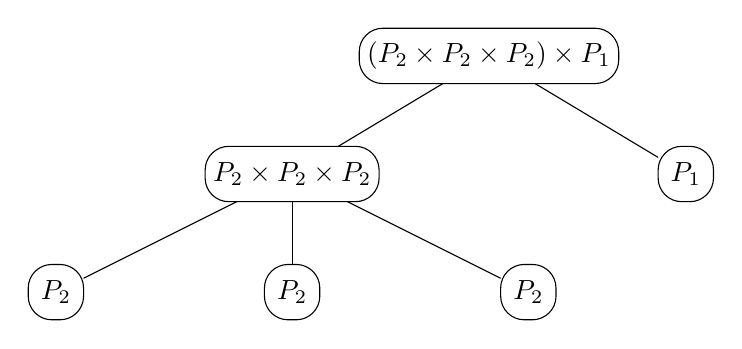
\begin{tikzpicture}[
                level/.style={
                    sibling distance = (3-#1)*2cm + 1cm,
                    level distance = 1.5cm
                }
            ]
            \node [treenode] {$(P_2\times P_2 \times P_2) \times P_1$}
                child{ node [treenode] {$P_2 \times P_2 \times P_2$}
                    child{ node [treenode] {$P_2$} }
                    child{ node [treenode] {$P_2$} }
                    child{ node [treenode] {$P_2$} }
                }
                child{ node [treenode] {$P_1$} };
        \end{tikzpicture}
    \end{center}
    \caption{Finite element tree of the Taylor--Hood space $(P_2 \times P_2 \times P_2)\times P_1$}
    \label{fig:taylor_hood_basis_tree}
\end{figure}

%\begin{figure}
%  \begin{center}
%   \begin{overpic}[width=0.5\textwidth]{taylor_hood_tree}
%    \put(5,5){$V_x$}
%    \put(30,5){$V_y$}
%    \put(55,5){$V_z$}
%    \put(87,31){$V_p$}
%    \put(5,30){$V_v$}
%    \put(5,57){$V_\text{TH}$}
%    \put(30.7,32){$\times$}
%    \put(61.6,58){$\times$}
%   \end{overpic}
%  \end{center}
%  \caption{Taylor--Hood basis $P_2 \times P_2 \times P_2 \times P_1$ in a tree representation}
%    \label{fig:taylor_hood_basis_tree}
%\end{figure}

While these extra nodes might initially appear like useless artifacts of the tree representation, they are often extremely useful
because we can treat the subtrees rooted in those nodes as individual trees in their own right, which often makes it possible to
reuse existing algorithms that expect to operate on those subtrees in more complex settings.




\subsection{Indexing basis functions by multi-indices}

To work with the basis of a finite element space, the basis vectors need to be indexed.  Indexing the basis functions
is what allows to address the corresponding vector and matrix coefficients in suitable vector and matrix data structures.
In simple cases, indexing means simply enumerating the basis functions with natural numbers, but for many applications
hierarchically structured matrix and vector data structures are more natural or efficient.  This leads to the need
for hierarchically structured multi-indices.

\begin{definition}
    \begin{enumerate}
        \item
            A tuple $I \in \N_0^k$ for some $k \in \N_0$ is called a multi-index of length $k$
            and we write $|I|=k$.
            The set of all multi-indices is denoted by
            $\mathcal{N} = \bigcup_{k \in \N_0^k} \N_0^k$.
        \item
            If $I \in \mathcal{N}$ takes the form $I = (I',I'')$ for $I',I'' \in \mathcal{N}$,
            then we call $I'$ a prefix of $I$ and write $I = (I',\dots)$.
            If additionally $|I''|>0$ we call $I'$ a strict prefix of $I$ and write $I = (I',*,\dots)$.
    \end{enumerate}
\end{definition}

Sets of multi-indices form trees as long as they are consistent in the sense that they
can be viewed as the paths to the leafs in an ordered tree.
%Consistency here means that the multi-indices should form an index tree.
That is, the children of each node are enumerated using consecutive zero-based
indices and paths to the leafs (i.e. the multi-indices) are build by concatenating
those indices starting from the root and ending in a leaf.

\begin{definition}
 A set $\mathcal{I} \subset \mathcal{N}$ is called an \emph{index tree}
 if for any $(I,i,\dots) \in \mathcal{I}$ there are also $(I,0,\dots),(I,1,\dots),\dots,(I,i-1,\dots) \in \mathcal{I}$
 but $I \notin \mathcal{I}$.
\end{definition}


We will illustrate this for the Taylor--Hood tree $(P_2 \times P_2 \times P_2) \times P_1$.
We start by assuming that the finite element basis functions $\lambda_i^2$ and $\lambda_k^1$
of $P_2$ and $P_1$ both
have a flat indexing by natural numbers $i=0,\dots,n_2$ and $k=0,\dots,n_1$,
respectively.
Then we enumerate the three children $P_2$, $P_2$, $P_2$
in the velocity subtree $P_2 \times P_2 \times P_2$
with the numbers $0$, $1$ and $2$.
Finally we enumerate the two children $(P_2 \times P_2 \times P_2)$ (for the velocity)
and $P_1$ (for the pressure) in the overall tree $(P_2 \times P_2 \times P_2) \times P_1$
with the numbers $0$ and $1$.
This construction leads to multi-indices of the form $[0,i,j]$ for velocity components, and $[1,k]$
for pressure components.
The left-most digit of the multi-index determines if the basis function
belongs to the velocity or pressure degrees of freedom.
For the velocity multi-indices $[0,i,j]$ the $i$ determines the component
of the velocity vector field and the $j$ determines the number of the scalar $P_2$ basis
function that determines this component.
For the pressure multi-indices $[0,k]$ the $k$ determines the number of the $P_1$ basis
function for the scalar $P_1$ function that determines the pressure.

It is important to note that the multi-indices for a given basis do not necessarily
have a fixed length.

If all basis functions $\lambda_I$ of the whole finite element tree are
indexed by multi-indices of the above given form,
and if $X$ is a coefficient vector that has a compatible hierarchical structure,
then the velocity vector field $u_h$ and the pressure field $p_h$ are given by
\begin{align*}
    u_h &= \bigg( \sum_{j=0}^{n_2} X_{(0,i,j)}\lambda_{(0,i,j)}\bigg)_{i=0,\dots,2},
    &
    p_h &= \sum_{k=0}^{n_1} X_{(1,k)}\lambda_{(1,k)}
\end{align*}
with basis functions
\begin{equation*}
    \lambda_{(0,i,j)} = \lambda^2_j \qquad i=0,1,2,
    \qquad \text{and} \qquad
    \lambda_{(1,k)} \lambda^1_k.
\end{equation*}

This index construction is illustrated in Figure~\ref{fig:taylor_hood_index_tree}
where the Taylor--Hood finite element tree is extended with individual basis functions,
edges are labels with corresponding multi-index entries, and node labels indicate
what the corresponding subtree represents.

\begin{figure}
    \begin{center}
        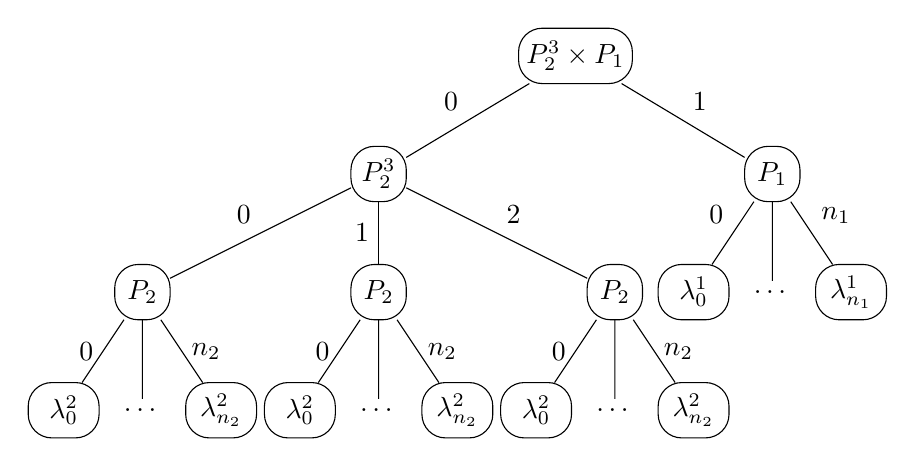
\begin{tikzpicture}[
                level/.style={
                    sibling distance = (3-#1)*2cm + 1cm,
                    level distance = 1.5cm
                }
            ]
            \node [treenode] {$P_2^3 \times P_1$}
                child{ node [treenode] {$P_2^3$}
                    child{ node [treenode] {$P_2$}
                        child{ node [basisnode] {$\lambda_0^2$} edge from parent node[left] {$0$}}
                        child{ node [] {$\dots$} }
                        child{ node [basisnode] {$\lambda_{n_2}^2$} edge from parent node[right] {$n_2$} }
                        edge from parent node[above left] {$0$}
                    }
                    child{ node [treenode] {$P_2$}
                        child{ node [basisnode] {$\lambda_0^2$} edge from parent node[left] {$0$}}
                        child{ node [] {$\dots$} }
                        child{ node [basisnode] {$\lambda_{n_2}^2$} edge from parent node[right] {$n_2$} }
                        edge from parent node[left] {$1$}
                    }
                    child { node [treenode] {$P_2$}
                        child{ node [basisnode] {$\lambda_0^2$} edge from parent node[left] {$0$}}
                        child{ node [] {$\dots$} }
                        child{ node [basisnode] {$\lambda_{n_2}^2$} edge from parent node[right] {$n_2$} }
                        edge from parent node[above right] {$2$}
                    }
                    edge from parent node[above left] {$0$}
                }
                child{ node [treenode] {$P_1$}
                    child [sibling distance=1cm] { node [basisnode] {$\lambda_0^1$} edge from parent node[above left] {$0$} }
                    child [sibling distance=1cm] { node [] {$\dots$} }
                    child [sibling distance=1cm] { node [basisnode] {$\lambda_{n_1}^1$} edge from parent node[above right] {$n_1$} }
                    edge from parent node[above right] {$1$}
                };
        \end{tikzpicture}
    \end{center}
    \caption{Index tree for Taylor--Hood with indices inherited from FE tree}
    \label{fig:taylor_hood_index_tree}
\end{figure}

In the previous example, the inner nodes of the index tree have formed a tree that was
isomorphic to the original basis tree.
However, one may also be interested in constructing multi-indices
that do not mimic the structure of the finite element tree:
To increase data locality in assembled matrices for the Taylor--Hood basis it may be
preferable to group all velocity degrees of freedom corresponding to a single
$P_2$ basis function together, i.\,e., to use the index $[0,j,i]$
for the $j$-the $P_2$ basis function for the $i$-th component.
The corresponding alternative index tree is illustrated in
Figure~\ref{fig:taylor_hood_index_blocked_tree}.
Figure~\ref{} shows the corresponding layouts of a hierarchical stiffness matrix.

\begin{figure}
    \begin{center}
        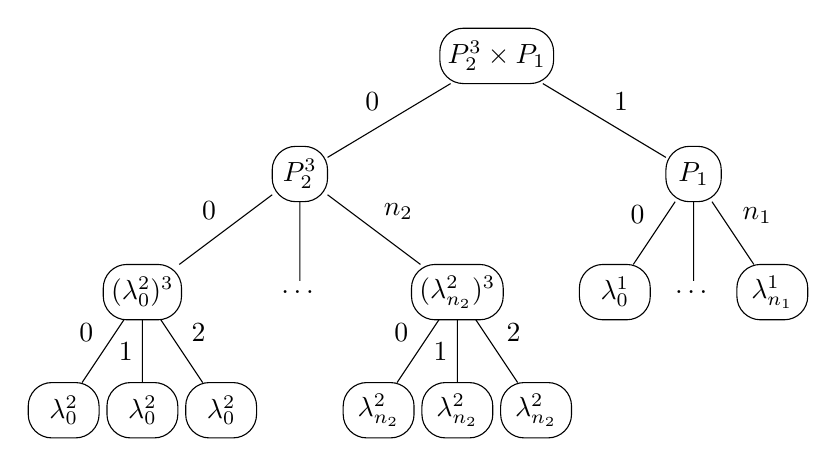
\begin{tikzpicture}[
                level/.style={
                    sibling distance = (3-#1)*2cm + 1cm,
                    level distance = 1.5cm
                },
            ]
            \node [treenode] {$P_2^3 \times P_1$}
                child{ node [treenode] {$P_2^3$}
                        child [sibling distance=2cm] { node [treenode] {$(\lambda_0^2)^3$}
                            child{ node [basisnode] {$\lambda_0^2$} edge from parent node[above left] {$0$}}
                            child{ node [basisnode] {$\lambda_0^2$} edge from parent node[left] {$1$}}
                            child{ node [basisnode] {$\lambda_0^2$} edge from parent node[above right] {$2$}}
                            edge from parent node[above left] {$0$}
                        }
                        child [sibling distance=2cm]{ node [] {$\dots$} }
                        child [sibling distance=2cm]{ node [treenode] {$(\lambda_{n_2}^2)^3$}
                            child{ node [basisnode] {$\lambda_{n_2}^2$} edge from parent node[above left] {$0$}}
                            child{ node [basisnode] {$\lambda_{n_2}^2$} edge from parent node[left] {$1$}}
                            child{ node [basisnode] {$\lambda_{n_2}^2$} edge from parent node[above right] {$2$}}
                            edge from parent node[above right] {$n_2$}
                        }
                        edge from parent node[above left] {$0$}
                }
                child{ node [treenode] {$P_1$}
                    child [sibling distance=1cm] { node [basisnode] {$\lambda_0^1$} edge from parent node[above left] {$0$} }
                    child [sibling distance=1cm] { node [] {$\dots$} }
                    child [sibling distance=1cm] { node [basisnode] {$\lambda_{n_1}^1$} edge from parent node[above right] {$n_1$} }
                    edge from parent node[above right] {$1$}
                };
        \end{tikzpicture}
    \end{center}
    \caption{Index tree for Taylor--Hood with blocking of local velocity components}
    \label{fig:taylor_hood_index_blocked_tree}
\end{figure}

\begin{figure}
 \begin{center}
   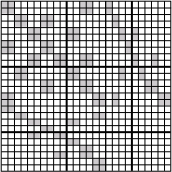
\includegraphics[width=0.4\textwidth]{taylor-hood-matrix-lexicographic}
   \qquad
   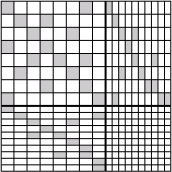
\includegraphics[width=0.4\textwidth]{taylor-hood-matrix-interleaved}
 \end{center}
 \caption{Two matrix occupation patterns.  Left: ordering the basis vectors of $B_x$, $B_y$, $B_z$, $B_p$
   one after the other gives a stiffness matrix with $4 \times 4$ sparse blocks.
   Right: interleaving the entries of $B_x$, $B_y$, $B_z$ gives a $2 \times 2$ block structure, where
   the entries are small blocks themselves.
   }
 \label{fig:matrix_occupation_patterns}
\end{figure}



If $\Lambda$ is the set of basis functions of a finite element tree,
then \dunemodule{dune-functions} allows any indexing scheme that
is given by an index map $I: \Lambda \to \mathcal{N}$
whose range $I(\Lambda)$ is an index tree.

When operating with the indices of basis functions it is important
to know the maximal appearing index in order to allocate matrices
and vectors.
For a flat consecutive zero-based index this is just $d-1$ where
$d$ is the dimension of the spanned space. For multi-indices from
an index tree $\mathcal{I}$ we need a slightly more complicated
construction. Let $(I,\dots) \in \mathcal{I}$, i.\,e., $I$ is a
prefix of multi-indices in $\mathcal{I}$ then the size relative
to $I$ is given by
\begin{align}\label{eq:prefix_size}
    |\mathcal{I}|_I = \op{max}\{k \st \exists (I,k,\dots) \in \mathcal{I} \}+1.
\end{align}
In terms of the ordered tree associated with $\mathcal{I}$ this corresponds
to the number of direct children of the node indexed by $I$.



\subsection{Rule-based construction of multi-indices}

While \dunemodule{dune-functions} allows to use arbitrary index trees
to enumerate the basis functions, there are some important generic constructions
to derive such index trees from the finite element tree.


\todosander{Rewrite this section to match the new section title}

There are two aspects to what we just have loosely called ``indexing''.  The first is that the set of all basis functions
in the tree need to be given a global order.  There are several reasonable choices to do this, which we discuss
in this section.
Given an order of the basis functions, there is then a natural indexing by simply enumerating the basis functions in
their specific order. This can be flat or hierarchical.

Consider first a leaf basis consisting of $n$ basis functions.  We suppose that these basis functions are given in a fixed
order (even though being able to change this ordering can improve the performance of a numerical
algorithm, see for example \cite{bader:2013,ordering_for_gauss_seidel} for more on this).
Consider now a tree of finite element bases with a given root $R$.  This root has $m$ children, and suppose that for
each of the subtrees rooted in these children we have already chosen an ordering.  Suppose further that the children themselves are given
in a fixed ordering (One may of course create different overall orderings by permuting the children, but in our view
this leads to a different bases, rather than to a different ordering of the same basis.)  It is then most natural
to first list all basis functions of the first tree, followed by all basis functions of the second subtree,
and so on.  This is the ordering obtained by a depth-first traversal of the tree~\cite{cormen:1990}.
For the Taylor--Hood basis with expression
\begin{equation*}
 B_\text{TH}
 =
 (B_x \otimes B_y \otimes B_z) \otimes B_p,
\end{equation*}
this means that the basis vectors are ordered as
\begin{equation*}
 b_{x,1}, b_{x,2}, \dots, b_{x,\abs{B_x}},
 b_{y,1}, \dots, b_{y,\abs{B_y}},
 b_{z,1}, \dots, b_{z,\abs{B_z}},
 b_{p,1}, \dots, b_{p,\abs{B_p}}.
\end{equation*}
(As this lists stands, but this has been done consciously to avoid overly technical notation.  Indeed, a given basis
function $b_{x,i}$ from the leaf basis is scalar valued.  However, in the product velocity space
$B_x \otimes B_y \otimes B_z$ the same basis function appears as $\mathbf{e}_1 b_{x,i} = (b_{x,i},0,0)^T$,
and now takes values in $\R^3$.  Furthermore, as part of the complete Taylor--Hood basis it is
$\tilde{\mathbf{e}}_1 b_{x,i} = (b_{x,i},0,0,0)^T$.  For the sake of the discussion here we identify a scalar
basis function $b_{x,i}$ with all of its vector-values variants.)

This is certainly a reasonable ordering.  Used in a finite element computation it will lead to a stiffness
matrix which, conceptually, consists of $4 \times 4$ large sparse blocks (Figure~\ref{fig:matrix_occupation_patterns}).
We call this the {\em lexicographic} ordering.

However, there is one important alternative.  Since, for the standard applications of the Taylor--Hood element,
the $B_x$, $B_y$, $B_z$ bases are used to discretize the $x, y, z$ components of a velocity vector field,
it would be rather unusual not to use identical bases for these three coefficients.
In this case, all three bases have the same number of basis functions with the same ordering.  We can therefore
{\em interleave} the basis functions from the three subtrees.  That is,
the basis functions of the Taylor--Hood basis appear in the order
\begin{equation*}
 b_{x,1}, b_{y,1}, b_{z,1},
 b_{x,2}, b_{y,2}, b_{z,2},
 \dots
 b_{x,N}, b_{y,N}, b_{z,N},
 b_{p,1}, \dots, b_{p\abs{B_p}}.
\end{equation*}
In this case, the stiffness matrix only has $2 \times 2$ large sparse blocks, but each entry of the uppler left
block will be a $3 \times 3$ matrix, each entry of the lower right block will be a scalar, and the off-diagonal
blocks will have a corresponding rectangular structure (Figure~\ref{fig:matrix_occupation_patterns}).

To deduce such possibilities from the tree structure we now divide the inner tree nodes into two classes.
An inner node will be called {\em power node}, if all of its children are identical subtrees.
An inner node that is not a power node is called {\em composite node}.  To construct an admissible ordering
of all basis functions in a tree we move recursively from the leaf nodes to the root.  To start the recursion,
the order of the basis functions in each leaf node is considered fixed.  At each inner node there are two
possibilities.
\begin{enumerate}
 \item The inner node is a composite node.  Then the basis functions of all the subtrees (with the ordering
   within each subtree already given by recursion) are concatenated to obtain lexicographic ordering.
   Remember that we suppose the order of the children to be fixed.
 %
 \item The inner node is a power node.  Then there are two choices: Either combine the subtree basis functions
   in lexicographic order, or interleave them.
\end{enumerate}
In total, for a tree with $N$ power nodes we obtain $2^N$ different ways to order the basis functions of the tree.



\begin{table}
 \begin{center}
 \begin{tabular}{c|c|c|c|c}
 \hline \\
  $b_{x,0}$  & $0$    & $(0,0)$ & $(0,0)$ & $(0,0,0)$ \\
  $b_{x,1}$  & $1$    & $(0,1)$ & $(0,1)$ & $(0,0,1)$ \\
  $b_{x,2}$  & $2$    & $(0,2)$ & $(0,2)$ & $(0,0,2)$ \\
    \vdots   & \vdots & \vdots  & \vdots  & \vdots  \\
  $b_{y,0}$  & $n$    & $(0,n)$ & $(1,0)$ & $(0,1,0)$ \\
  $b_{y,1}$  & $n+1$  & $(0,n+1)$ & $(1,1)$ & $(0,1,1)$ \\
  $b_{y,2}$  & $n+2$  & $(0,n+2)$ & $(1,2)$ & $(0,1,2)$ \\
    \vdots   & \vdots & \vdots  & \vdots  & \vdots  \\
  $b_{z,0}$  & $2n$   & $(0,2n)$ & $(2,0)$ & $(0,2,0)$ \\
  $b_{z,1}$  & $2n+1$ & $(0,2n+1)$ & $(2,1)$ & $(0,2,1)$ \\
  $b_{z,2}$  & $2n+2$ & $(0,2n+2)$ & $(2,2)$ & $(0,2,2)$ \\
    \vdots   & \vdots & \vdots  & \vdots  & \vdots  \\
  $p_0$      & $3n$   & $(1,0)$ & $n$ & $(1,0)$ \\
  $p_1$      & $3n+1$ & $(1,1)$ & $n+1$ & $(1,1)$ \\
  $p_2$      & $3n+2$ & $(1,2)$ & $n+2$ & $(1,2)$ \\
    \vdots   & \vdots & \vdots  & \vdots  & \vdots
 \end{tabular}
 \end{center}
 \caption{Possible index types for a Taylor--Hood basis with lexicographic ordering of the velocity basis functions}
 \label{tbl:th_multiindices_lexicographic}
\end{table}

\begin{table}
 \begin{center}
 \begin{tabular}{c|c|c|c|c}
 \hline \\
  $b_{x,0}$  & $0$    & $(0,0)$ & $(0,0)$ & $(0,0,0)$ \\
  $b_{y,0}$  & $1$    & $(0,1)$ & $(0,1)$ & $(0,0,1)$ \\
  $b_{z,0}$  & $2$    & $(0,2)$ & $(0,2)$ & $(0,0,2)$ \\
  $b_{x,1}$  & $3$    & $(0,3)$ & $(1,0)$ & $(0,1,0)$ \\
  $b_{y,1}$  & $4$    & $(0,4)$ & $(1,1)$ & $(0,1,1)$ \\
  $b_{z,1}$  & $5$    & $(0,5)$ & $(1,2)$ & $(0,1,2)$ \\
  $b_{x,2}$  & $6$    & $(0,6)$ & $(2,0)$ & $(0,2,0)$ \\
  $b_{y,2}$  & $7$    & $(0,7)$ & $(2,1)$ & $(0,2,1)$ \\
  $b_{z,2}$  & $8$    & $(0,8)$ & $(2,2)$ & $(0,2,2)$ \\
    \vdots   & \vdots & \vdots  & \vdots  & \vdots  \\
  $p_0$      & $3n$   & $(1,0)$ & $n$ & $(1,0)$ \\
  $p_1$      & $3n+1$ & $(1,1)$ & $n+1$ & $(1,1)$ \\
  $p_2$      & $3n+2$ & $(1,2)$ & $n+2$ & $(1,2)$ \\
    \vdots   & \vdots & \vdots  & \vdots  & \vdots
 \end{tabular}
 \end{center}
 \caption{Possible index types for a Taylor--Hood basis with interleaved ordering of the velocity basis functions
 \todo[inline]{Inkonsistenz:  Der Index in der rechten Spalte ist so wie man ihn als Programmierer erwarten würde.
   Aus Sicht der Baumkonstruktion ist er allerdings inkonsequent.  Der skalare Index in einer einzelnen Blatt-Basis
    erscheint nicht als letzte Stelle im Multi-Index, sondern als {\em vorletzte}.  Das muss man ordentlich
    begründen, und schauen was in allgemeineren Bäumen passiert.}
 \label{tbl:th_multiindices_interleaved}
 }
\end{table}

\subsection{Localization to single elements}

For the most part, access to finite element bases happens element by element.  It is therefore important
to consider the restrictions of bases to single grid elements.  In contrast to the previous sections
we now require that all bases in a given tree are defined with respect to the same grid.
\todosander{Ist das übertrieben restriktiv? Es würde ja reichen wenn es ein ausgezeichnetes Gitter gäbe,
  bzgl.\ dem man lokalisieren kann. Den Fall hätte man zum Beispiel wenn man normale FE mit
  Fourier-Basen kombinieren will.}

We now consider the restrictions of all basis functions of a given tree to a single fixed grid element $e$.
Of these restricted functions, we discard all those that are constant zero functions on $e$.
All others form the \emph{local basis} on $e$
\begin{equation*}
 \Lambda_\text{local}
 \colonequals
 \{ \lambda|_e \; : \; \lambda \in \Lambda \}.
\end{equation*}
The local basis forms a tree that is isomorphic to the full global basis tree.
\todosander{Das ist unpräzise: Die Aussage gilt nur, wenn man den Baum betrachtet, in dem
  die Blätter die irreduziblen Basen sind, \emph{nicht} die einzelnen Basisfunktionen.}

The basis functions in the local tree have two indices in addition to the global one.
First, each local basis function has an index to distinguish it from other functions in the
same leaf node.  As there is no hierarchical structure involved, this index is simply a
natural number.
\todosander{Hat diese Nummer einen Namen?}
Secondly, each local basis has an index for the entire local tree.  This is what is used to address
the element stiffness matrix.
\todosander{Hat diese Nummer einen Namen?}
In principle, this indexing can use another general index tree, which does not have to coincide
with the index tree for the global basis.
\todosander{Die Implementierung nimmt zwar aktuell immer nur flache Indizes, aber ich bin dennoch
 versucht das hier in voller Allgemeinheit aufzuschreiben.  Er im Kapitel zum API würde ich dann
 sagen dass der Index immer flach ist.  Ein Grund ist, dass wir ja selbst ab und zu noch mit
 der Festlegung auf flache Indizes hadern.}


\section{Programmer interface for function space bases}
\label{sec:function_space_bases_implementation}

The design of the \dunemodule{dune-functions} interfaces for bases of discrete function spaces
follows the ideas of the previous section. The main interface concept are global basis objects
that represent trees of function space bases. These trees can be localized to individual elements
of the grid.  Such a localization gives you access to the (tree of) shape functions there,
and it provides the three types of shape-function indices.

\begin{figure}
 \begin{center}
  \begin{overpic}[width=\textwidth]{febasis_interface_schematic}
  \put(54.5,37){$\times$}
  \put(49,32){$\times$}
  \put(60,32){\tiny $P_1$}
  \put(44,27){\tiny $P_2$}
  \put(49,27){\tiny $P_2$}
  \put(54,27){\tiny $P_2$}
  \end{overpic}
 \end{center}
 \caption{Overview of the classes making up the interface to finite element space bases}
 \label{fig:febasis_interface_schematic}
\end{figure}

The user interface of localized function space bases is divided into two parts.  A \cpp{LocalView} on an
element allows you to obtain the (tree of) local basis functions of that element, which in turn gives you access to all
shape functions, associations to element subentities, and local interpolation rules provided by
\dunemodule{dune-localfunctions}.  A local view is attached to a particular grid element by an
action called \emph{binding}.
The mapping of these shape functions to global degrees of freedom is
delegated to a separate object called a \cpp{LocalIndexSet}, which you can bind to given
\cpp{LocalView} objects.  Once bound, a \cpp{LocalIndexSet} will provide global (multi-)indices
for each shape function on this element, and flat indices with respect to the local tree.
The structure of the interface is visualized in
Figure~\ref{fig:febasis_interface_schematic}.

All header include paths
start with \cpp{dune/functions/}, and all code is contained in the namespace \cpp{Dune::Functions}.
Internally, \dunemodule{dune-functions} depends on the \dunemodule{dune-typetree} module,
which implements abstract compile-time tree data structures.
The global basis interface described below is not enforced by deriving
from specific base classes. Instead, \dunemodule{dune-functions} is based on
duck-typing,
\todosander{Referenz}
i.e., any object providing the required
interface is a valid global basis.



\subsection{User interface of a \cpp{GlobalBasis}}
We start by describing the user interface of global bases.  Since we are discussing duck-typing interfaces,
all class names used below are generic. Trees of global bases are implemented by classes that implement
the \cpp{GlobalBasis} interface. In the following, we will call the generic such class \cpp{GlobalBasis}.
It can have an arbitrary number of template parameters.
In the following interface description such implementation details
are marked by the placeholder \cpp{@@<implementation defined>@@}.

In general each basis implementation may require its own specific data for construction.
Hence we do not enforce an argument list for this.
\begin{lstlisting}[style=Interface]
GlobalBasis(@@<implementation defined>@@);
\end{lstlisting}
The global basis represents a function space defined on a grid view, and access to
this view is provided by the
\begin{lstlisting}[style=Interface]
const GridView& gridView() const;
\end{lstlisting}
method. The corresponding type
is exported as \cpp{GridView}. If the grid view
was modified (e.g., by local grid refinement), the result of calling any
method of the basis is undefined until the basis was updated by
providing a new grid view by the method
\begin{lstlisting}[style=Interface]
void update(const GridView & gv);
\end{lstlisting}
\todosander{Die \cpp{update}-Methode wird noch nicht vom Standard-Test getestet!}

Access to the basis functions is available via the
local view interface.
\begin{lstlisting}[style=Interface]
using LocalView = @@<implementation defined>@@;
LocalView localView() const;
\end{lstlisting}
The \cpp{localView()} method returns a new object that implements the \cpp{LocalView} interface.
After binding this object to a
grid element from the respective grid view, it provides access
to the restriction of all basis functions whose support has a
nontrivial intersection with this element.  With a global basis given in an object called \cpp{basis},
the corresponding code is
\begin{lstlisting}[style=Example]
auto localView = basis.localView();
localView.bind(element);
\end{lstlisting}
where \cpp{element} is an element from the grid view.
For details on the
\cpp{LocalView} interface see below.

To access the various types of indices of a shape function,
the \cpp{localIndexSet()} method
returns a new object of type \cpp{LocalIndexSet} that, after
binding it to a local view, allows to map the local indices
of all basis functions appearing in this local view to those
global multi-indices.
\begin{lstlisting}[style=Interface]
using LocalIndexSet = @@<implementation defined>@@;
LocalIndexSet localIndexSet() const;
\end{lstlisting}
The interface of the \cpp{LocalIndexSet} is discussed in Section~\ref{sec:localindexset_interface}.

An additional group of methods provides information on the sizes of the bases
contained in the tree.
The total number of basis functions of the global basis is
exported via the \cpp{dimension()} method. However, since
the global indices are hierarchically structured multi-indices,
this information is generally not
sufficient to allocate hierarchical containers for storing,
e.g., coefficients with respect to all basis functions.
Therefore, the basis provides access to the structural
information of those multi-indices via the \cpp{size(SizePrefix)}
method. The given prefix takes the form of a multi-index itself.
If $\mathcal{I}$ is the set of all global multi-indices of the
basis and $P \in \mathcal{N}$ is a prefix for this set,
i.e. there is a $(P,\dots) \in \mathcal{I}$, then
\cpp{size(P)} returns the size $|\mathcal{I}|_P$ of
$\mathcal{I}$ relative to $P$ defined according to \eqref{eq:prefix_size}.
%For a prefix $(p_1,\dots,p_k)$ the method returns the maximal value $q$ such that there
%is a global index of the form $(p_1,\dots,p_k,q-1,\dots)$.
If $P$ is not a prefix for $\mathcal{I}$ the result is undefined.
If $P \in \mathcal{I}$, i.e., the prefix is itself one of the multi-indices
then the result is zero.
In any case the result corresponds to the number of direct children
of the node $P$ in the index tree.
For convenience there is also a method \cpp{size()} returning the same
value as the method with an empty prefix, i.e., \cpp{size(\{\})}.
For a scalar basis, this method again returns the number of basis functions.

\todosander{Irgendwo muss der Typ (bzw.\ das Konzept) \cpp{MultiIndex} erklärt werden.}

Since prefixes may have variable size, it is guaranteed that the type \cpp{SizePrefix}
is always a \cpp{Dune::ReservedVector<size\_type,k>} where \cpp{k}
is strictly larger than the maximal length of a multi-index. The result
type of all size-related methods is exported as \cpp{size\_type}.
\todograeser{Do we need 'strictly larger'? As far as I can see 'at least' should be OK.}
\todosander{An manchen Stellen im Code hat man tatsächlich eine Stelle mehr als die
Länge des längsten MultiIndex (zB \cpp{LagrangeDGBasis}).  Darüber habe ich mich auch
schon gewundert.}

\begin{lstlisting}[style=Interface]
using size_type = @@<implementation defined>@@;
using SizePrefix = @@<implementation defined>@@;
using MultiIndex = @@<implementation defined>@@;
size_type dimension() const;
size_type size() const;
size_type size(const SizePrefix& prefix) const;
\end{lstlisting}

\todosander{Wollen wir eventuell ein separates Unterkapitel für diese Teilbaumkonstruktionen
machen?  Hier an dieser Stelle finde ich die Erklärungen etwas verwirrend.}

Additionally to the concept of a global basis as defined here, there
is also the concept of a so called \cpp{SubspaceBasis} reflecting
the basis of the subtree only spanned by those basis functions
associated to a subtree of the local ansatz tree of the so-called
root basis.
For convenience a global basis behaves like a trivial \cpp{SubspaceBasis},
i.e., the method \cpp{rootBasis()} returns the basis itself
and \cpp{prefixPath()} returns an empty tree-path of the
implementation defined type \cpp{PrefixPath}.
\todograeser{While describing the interface I had the impression that having
those methods here is inconsistent and that they should maybe be free functions.}
\todosander{Könnte man tatsächlich in Betracht ziehen.}

\begin{lstlisting}[style=Interface]
using PrefixPath = @@<implementation defined>@@;
const @@<implementation defined>@@& rootBasis() const
const PrefixPath& prefixPath() const
\end{lstlisting}

Finally, the basis exports its pre-basis of type \cpp{PreBasis}
via the \cpp{preBasis()} method. The concept of a pre-basis
will be discussed in Chapter~\ref{sec:implementation_api}.
\todograeser{%
    Do we require that \cpp{preBasis()} and \cpp{PreBasis} exists?
    Do we require that each global basis is implemented using a pre-basis?
    Do we require that GlobalBasis is always a DefaultGlobalBasis parametrized with the pre-basis?
}
\todosander{I'd say we require that any basis can become part of a tree.
  If that means that each global basis needs to be implemented using a factory: so be it.}
\todograeser{Update: The above given questions are the topic of
\url{https://gitlab.dune-project.org/staging/dune-functions/issues/4}
and were discussed on the last meeting. There we had some consensus,
that it would be nice if any global basis is reusable but that we
do not require this. Hence the answer to all three questions above is 'no'.
}

\begin{lstlisting}[style=Interface]
using PreBasis = <implementation define>;
const PreBasis& preBasis() const;
\end{lstlisting}


To statically check for the interface,
\dunemodule{dune-functions} provides a concept definition of a global
basis which can, e.g., be used to check validity in a static assertion.

\begin{lstlisting}[style=Example]
// The global basis concept for given grid view
using GlobalBasisConcept = Dune::Functions::Concept::GlobalBasis<GridView>;

// Check if Basis models the concept
static_assert(Dune::models<GlobalBasisConcept, Basis>(),
  "Basis does not model the global basis concept.")
\end{lstlisting}

\subsection{User interface of a \cpp{LocalView}}

The \cpp{LocalView} concept represents the localization of a basis tree to a single element.
\cpp{LocalView} objects are returned by the method \cpp{GlobalBasis::localView()}.
There is no way to construct such objects directly.
The global basis of type \cpp{GlobalBasis}
is known by the \cpp{LocalView} object, and exported by the \cpp{globalBasis()} method.
\begin{lstlisting}[style=Interface]
using GlobalBasis = @@<implementation defined>@@;
const GlobalBasis& globalBasis() const;
\end{lstlisting}

A local view provides access to all basis
functions whose support has nontrivial intersection with
a given element (the \emph{local basis functions}).
To achieve this, the local view must
first be bound to this element by calling
\begin{lstlisting}[style=Interface]
using GridView = typename GlobalBasis::GridView;
using Element = typename GridView::template Codim<0>::Entity;
void bind(const Element& e);
\end{lstlisting}
This call may incorporate expensive computations needed to
setup the those local basis functions. The local view can be
bound to another element by calling this method again.
To set the local view to unbound state again, you
can call the
\begin{lstlisting}[style=Interface]
void unbind();
\end{lstlisting}
method.
Notice that the local view will store a copy of the bound
element that is accessible via \cpp{element()}.
\begin{lstlisting}[style=Interface]
using Element = typename GridView::template Codim<0>::Entity;
const Element& element() const;
\end{lstlisting}

The total number of basis functions associated to the
local view at the currently bound element is returned
by \cpp{size()}. The result of calling this method in
unbound state is undefined.
To allow preallocation of buffers for local functions
the \cpp{maxSize()} method returns the maximum of the
\cpp{size()} method for all elements in the grid view
associated to the global basis. This can be called in
unbound state.

\begin{lstlisting}[style=Interface]
using size_type = typename GlobalBasis::size_type;
size_type size() const;
size_type maxSize() const;
\end{lstlisting}

Finally access to the actual local basis functions are provided
by the \cpp{tree()} method returning a reference to a
\cpp{Tree} object. This encapsulates the basis functions
in a hierarchical tree structure to also represent structured
function spaces.
While the tree  itself can be queried in unbound state,
the local view must be bound in order to use most of the
trees methods.
A detailed discussion of the interface of the tree object is
given below.

\begin{lstlisting}[style=Interface]
using Tree = @@<implementation defined>@@;
const Tree& tree() const;
\end{lstlisting}

\todosander{Siehe oben: Für den Krams zu Teilraumbasen würde ich ein separates Unterkapitel einführen.}
In order to be consistent with a \cpp{SubspaceBasis::LocalView}
the additional method \cpp{rootLocalView()} returns the local view
itself.
\todograeser{While describing the interface I had the impression that having
this method here is inconsistent and that it should maybe be a free function.}

\begin{lstlisting}[style=Interface]
const DefaultLocalView& rootLocalView() const
}; // end LocalView
\end{lstlisting}

\subsection{User interface of a local ansatz \cpp{Tree}}
The local view provides access to all local basis functions
by exporting a \cpp{Tree} object. This implements a tree
data structure using the foundation classes of the
\dunemodule{dune-typetree} library, where the actual local basis
functions for each factor are associated to a leaf node
in the tree. As a consequence the interface of leaf nodes
provides some additional features.
Both node types are not meant to be constructed by the
user so there is no constructor in the interface.
First we describe the interface shared by interior
and leaf nodes.

The \cpp{size()} method returns the total number of
local basis functions within the subtree rooted at the
present node. For each of these local basis functions
the \cpp{localIndex(size\_type)} method returns a unique
local index within all local basis functions associated to the full
tree. The argument to this method is the lexicographic
index of the local basis functions within the subtree
and the result is the lexicographic index within the full
tree. Hence the local indices of all basis functions
within this subtree form a consecutive range. The first
value in this range, i.e., the result of \cpp{localIndex(0)}
is also accessible via the \cpp{offset()} method.
The result of these methods is undefined if the
local view containing the tree is in unbound state.
All these indices are of type \cpp{size\_type}.
\todograeser{Is the offset() method part of the interface?
Making it protected seems to be reasonable.}

\begin{lstlisting}[style=Interface]
class BasisNode
{
public:
using size_type = @@<implementation defined>@@;
size_type size() const;
size_type offset() const;
size_type localIndex(size_type i) const;
\end{lstlisting}

For some computations it is important to identify
individual nodes in the tree. To this end the node
exports its path in the full tree via the \cpp{treePath()}
method. The result is a tree path
as defined in the \dunemodule{dune-typetree} module.
It is possible to retrieve the node from the full
tree by addressing it with its tree path.
Notice that, to allow this functionality, the
type \cpp{TreePath} will in general differ from one node to the other.
If data needs to be attached to nodes,
the \cpp{treeIndex()} can be used. The latter returns
the lexicographic index of the node within the full
tree in a fixed type for all nodes.
These methods can also be used if the local view containing
the tree is in unbound state.

\begin{lstlisting}[style=Interface]
using TreePath = @@<implementation defined>@@;
const TreePath& treePath() const;
size_type treeIndex() const;
}; // end BasisNode
\end{lstlisting}

Leaf nodes share the same interface as interior
nodes. Additionally they provide access to the
element which the local view and thus the tree is bound
to via the \cpp{element()} method. Probably most important
is the \cpp{finiteElement()} method that gives access
to the local finite element. The finite element
itself provides access to the local basis functions
by the finite element interface defined in the
\dunemodule{dune-localfunctions} module.
It is important to note that the lexicographic
index of a basis function in a leaf node coincides
with its number in the local finite element.

\begin{lstlisting}[style=Interface]
class LeafBasisNode
{
public:
// interface common with interior nodes
using size_type = @@<implementation defined>@@;
size_type size() const;
size_type offset() const;
size_type localIndex(size_type i) const;
using TreePath = @@<implementation defined>@@;
const TreePath& treePath() const;
size_type treeIndex() const;

using Element = @@<implementation defined>@@;
using FiniteElement = @@<implementation defined>@@;
const Element& element() const = 0;
const FiniteElement& finiteElement() const = 0;
}; // end LeafBasisNode
\end{lstlisting}



\subsection{User interface of a \cpp{LocalIndexSet}}
\label{sec:localindexset_interface}

The \cpp{LocalIndexSet} as returned by \cpp{GlobalBasis::localIndexSet()}
provides access to global multi-indices for the
local basis functions reachable from a local view.
To this end the \cpp{LocalIndexSet} must
first be bound to the \cpp{LocalView} using
the \cpp{bind(LocalView)} method. Similar to the
local view there is an \cpp{unbind()} method
and the bound-to local view can be accessed
using the \cpp{localView()} method.
Notice that the \cpp{bind(LocalView)} operation
can be costly, because it pre-computes
all global indices and stores them in an internal cache.

\begin{lstlisting}[style=Interface]
class LocalIndexSet
{
public:
using LocalView = @@<implementation defined>@@;
const LocalView& localView() const;
void bind(const LocalView& localView);
void unbind();
\end{lstlisting}

If the local index set is in bound state
the \cpp{size()} method can be used to query
the number of local basis functions in the
bound local view. This is a simple shortcut for
\cpp{localView().size()} and \cpp{localView().tree().size()}.
For any of these local basis functions the global
multi-index is provided by the \cpp{index(size\_type)}
method. The argument for this method is the local
index of the basis function within the tree as
returned by the \cpp{BasisNode::localIndex(size\_type)}
method.
Accessing the same global index multiple times
is cheap, because global indices are pre-computed
and cached during \cpp{bind(LocalView)}.

\begin{lstlisting}[style=Interface]
using MultiIndex = @@<implementation defined>@@;
using size_type = @@<implementation defined>@@;
size_type size() const;
MultiIndex index(size_type i) const;
}; // end LocalIndexSet
\end{lstlisting}

We now give a short example on how to use the interface
to compute global indices for local basis functions
of a given \cpp{globalBasis} at a given \cpp{element}.
If we want to compute the global index of the \cpp{i}-th
local basis function in the finite element attached to
a leaf node this can be done by the following snippet.

\begin{lstlisting}[style=Example]
// create a LocalView and a LocalIndexSet
auto localView = basis.localView();
auto localIndexSet = basis.localIndexSet();

// bind the LocalView to the element and the LocalIndexSet to the LocalView
localView.bind(element);
localIndexSet.bind(localView);

// obtain the basis tree
const auto& node = localView.tree();

// compute local index of local basis function within the tree
auto localIndex = node.localIndex(i);

// compute global index of local basis function
auto globalIndex = localIndex.index(localIndex);
\end{lstlisting}

Here we assumed that we do not have a nested local ansatz tree
such that the \cpp{tree()} method directly returns a \cpp{LeafBasisNode}.
In this case \cpp{localIndex} coincides with \cpp{i}.
In the more general case of a nontrivial product space
we must first retrieve the leaf node corresponding to
the desired factor in the product space. This can be done
using the tree path for this node. If, for example,
we have a Taylor-Hood element, where the first
child in the tree corresponds to the velocity,
which itself has $dim$ children for the velocity
components, the leaf node for the second velocity
component can be obtained by the following.

\begin{lstlisting}[style=Example]
// import namespace with index constants
using namespace Indices;

// generate tree path for 2nd component of the velocity tree
auto treePath = TypeTree::hybridTreePath(_0, 1);

// obtain the desired leaf node in the basis tree
const auto& node = TypeTree::child(localView.tree(), treePath);
\end{lstlisting}

Notice that we used the index constants \cpp{\_0}
from the namespace \cpp{TypeTree::Indices}
to address the velocity node because the
tree root is a hybrid container whose child nodes
for velocity and pressure are of different type.
The same result can be achieved by the following
slightly more compact code.

\begin{lstlisting}[style=Example]
// import namespace with index constants
using namespace Indices;

// obtain the desired leaf node in the basis tree
const auto& node = localView.tree().child(_0, 1);
\end{lstlisting}




\subsection{Function space bases available in \texorpdfstring{\dunemodule{dune-functions}}{dune-functions}}
\label{subsec:available_bases}

The \dunemodule{dune-functions} module contains a collection of finite element bases that implement
this interface.  At the time of writing these are:

\begin{itemize}
 \item \cpp{PQkNodalBasis}: Lagrangian bases of order $k$, where $k$ is a compile-time parameter.
   For $k\le 2$, this implementation works on all kinds of conforming grids, including grids with more
   than one element type.  At the time of writing, higher-order spaces are implemented only partially.
   Check the online class documentation for the current status.

 \item \cpp{PQ1NodalBasis}: Lagrangian nodal bases of first order.  This is a separate implementation of
   the case $k=1$ of the previous basis.  It exists mainly so that people interested in writing their
   own bases have a simple example to look at.

 \item \cpp{TaylorHoodBasis}: The Taylor--Hood bases described in Chapter~\ref{sec:finite_element_trees}.
   This is a simple example of basis constructed by building products.
   A complete example for how to use this basis is given in Chapter~\ref{sec:stokes_example}.
   \todosander{Sollen wir diese Basis komplett entfernen, wo man sie mittlerweile doch
     einfach aus den Einzelteilen zusammenbasteln kann?}
   \todograeser{Es war Christian wichtig, dass man nicht-triviale Basen auch manuell,
    d.h. ohne \cpp{PowerPreBasis}, implementieren kann. Für diesen Fall taugt
    das noch als Beispiel.}

 \item \cpp{LagrangeDGBasis}: Implements a $k$-th order Discontinuous-Galerkin basis with Lagrange shape functions.
   The shape functions are the same as for the \cpp{PQkNodalBasis},
   but the basis functions are not continuous across the element boundaries.  Therefore, this basis also
   works well on non-conforming grids.  The polynomial order is again a compile-time constant.

 \item \todosander{Raviart--Thomas basis}

 \item \todosander{Rannacher--Turek basis}

 \item \todosander{BDM basis}

 \item \cpp{BSplineBasis}:  Implements a $B$-Spline basis on a structured, axis-aligned grid as described,
   e.g., in~\cite{cottrell_hughes_bazilevs:2009}.  Arbitrary orders, dimensions, and knot vectors are supported,
   allowing, e.g., to work with $C^1$ elements for fourth-order differential equations.

   Each \cpp{BSplineBasis} object implements a basis on a single patch, and the grid must correspond to this
   patch. For this to work, several restrictions apply for the grid.  It must be structured and axis-aligned,
   and consist of (hyper-)cube elements only.  Further, the element indices must be lexicographic and
   increase from the lower left to the upper right domain corner.  The element spacing must match the knot spans.
   Unfortunately, not all these requirements can be checked for by the basis, so users have to be a bit
   careful.  Using a \cpp{YaspGrid} object works well.

   Note that unlike in standard finite element bases, in a B-spline basis the basis functions cannot be associated
   to grid entities such as vertices, edges, or elements.  The interface nevertheless mandates that a
   \cpp{LocalCoefficient} object must be available, but for the \cpp{BSplineBasis}, the behavior of this
   object is undefined.
\end{itemize}

\todosander{Wir müssen hier beschreiben dass selbst Basen für nicht-affine FE immer nur
  Größen zurückgeben, die sich auf das Referenzelement beziehen.}

\subsection{Combining bases into trees}

The basis implementations of the previous section can be combined by external summation to form new bases.
This produces the tree structure described in Section~\ref{sec:finite_element_trees}.
The code for this resides in the \cpp{BasisBuilder} namespace, which is a nested namespace
within \cpp{Dune::Functions::}. Therefore, the examples of this section need a
\begin{lstlisting}[style=Example]
using namespace Dune::Functions::BasisBuilder;
\end{lstlisting}
to compile.

The methods to combine bases into trees do not operate on the basis classes of the previous section
directly.  Rather, they combine so-called \emph{pre-bases}, of which there is one for each basis.
The reason for this is
that it is technically very challenging to combine the actual user-visible basis types in a
tree hierarchy that itself again implements the interface of a hierarchical function space basis.
The pre-basis of the final basis tree can then be turned into an actual basis by a call to
\begin{lstlisting}[style=Interface]
template <class GridView, class PreBasisFactory>
auto makeBasis(const GridView& gridView, PreBasisFactory&& preBasisFactory);
\end{lstlisting}
This method takes a pre-basis factory, and produces a complete basis from it.

In the simple-most case, the tree consists of a single basis. That means that in particular
you can write
\todosander{\cpp{rt} ist als Abkürzung arg kurz -- sollten wir ändern!}
\todosander{Darf nicht mehr \cpp{BasisType} benutzen!}
\begin{lstlisting}[style=Example]
auto raviartThomasBasis = makeBasis(gridView, rt<k, GeometryType::BasicType::cube>());
\end{lstlisting}
to obtain a Raviart--Thomas basis for the given grid view.  This is equivalent to constructing
the basis directly:
\todosander{Ja, das Ding hat tatsächlich ``\emph{nodal}'' im Namen.  Sollten wir die Basis-Klasse
nicht einfach \cpp{RaviartThomasBasis} nennen?}
\begin{lstlisting}[style=Example]
RaviartThomasNodalBasis<GridView,k,GeometryType::BasicType::cube> raviartThomasBasis;
\end{lstlisting}
\todosander{Was passiert wenn ich eine Basis nicht mit dem Default-Konstruktor erzeugen möchte?
  Kann ich der \cpp{PreBasisFactory} dann Argumente mitgeben?}
\todograeser{Genau, die \cpp{PreBasisFactory} bekommt alle Basis-spezifischen Argumente aber
 verzögert die Erzeugung der \cpp{PreBasis}. \cpp{makeBasis()} reicht dann die fehlenden Argumente weiter
 und erzeugt mit \cpp{PreBasisFactory::makePreBasis<MultiIndex>(gridView)} die \cpp{PreBasis}. D.h. Unterstützung für
 zusätzliche Argumente muß man in \cpp{FooPreBasisFactory} und \cpp{foo()} implementieren.}

Each basis implementation listed above has a corresponding pre-basis factory, defined in the same header.
Some of them have template parameters to transmit compile-time information.  The factories are
\todosander{Die folgende Liste muss noch vervollständigt werden.}
\begin{center}
 \begin{tabular}{r|r}
  Basis & tag \\
  \hline
  \cpp{RaviartThomasNodalBasis} & \cpp{rt} \\
  \dots & \dots
 \end{tabular}
\end{center}

The general mechanism to combine bases in a tree is called \cpp{composite},
defined in the header \file{dune/functions/functionspacebases/compositebasis.hh}.
The composite mechanism consists of a single method
\begin{lstlisting}[style=Interface]
template <typename... Args>
auto composite(Args&&... args);
\end{lstlisting}
The method has an unspecified number of arguments, of unspecified type. The arguments are expected
to be either factory tags for basis objects, like \cpp{lagrange<1>()}, \cpp{rt<k, GeometryType::BasicType::cube>()},
or they can be the return value of another call to the \cpp{composite} method (or the \cpp{power} method,
see below).  They are the subtrees of a new function space basis tree, and the call to \cpp{composite}
adds the new tree root.

As an example, to combine a Raviart--Thomas basis with a zero-order Lagrange basis (for solving
the mixed formulation of the Poisson equation, say), the appropriate call is
\todosander{\cpp{pq} sieht auch blöd aus.  Können wir das, z.B., \cpp{lagrange} nennen?
  Update: Oh, scheint irgendwie auch zu gehen.}
\begin{lstlisting}[style=Example]
auto mixedBasis = makeBasis(
  gridView,
  composite(
    rt<0, GeometryType::BasicType::cube>(),
    pq<0>()
  ));
\end{lstlisting}
Combining three copies of a Lagrange basis for a displacement field in elasticity theory is
\begin{lstlisting}[style=Example]
auto displacementBasis = makeBasis(
  gridView,
  composite(
    pq<1>(),
    pq<1>(),
    pq<1>()
  ));
\end{lstlisting}
The examples produce the trees shown in Figure~\ref{fig:composite_example_bases}.

That last example is not as elegant as it could be.  First of all, it is inconvenient and unnecessarily
wordy to list the same scalar Lagrange basis three times.  Also, the required number may depend on
a compile-time parameter. Thirdly, in that case
more ways of degree-of-freedom numbering is possible. For these reasons, \dunemodule{dune-functions}
offers a second way to combine bases called \cpp{power}.  The interface is again a single method
\begin{lstlisting}[style=Interface]
template<std::size_t k, class ChildPreBasisFactory>
auto power(ChildPreBasisFactory&& childPreBasisFactory)
\end{lstlisting}
provided in the file \file{dune/functions/functionspacebases/powerbasis.hh}.
It combines \cpp{k} copies of a subtree of type \cpp{ChildPreBasisFactory} in a new tree.  Therefore, the
displacement vector field from above is more easily written as
\begin{lstlisting}[style=Example]
auto displacementBasis = makeBasis(
  gridView,
  power<3>(
    pq<1>()
  ));
\end{lstlisting}
Of course, all these techniques can be combined. To obtain the \cpp{p}-th order Taylor--Hood basis,
write
\begin{lstlisting}[style=Example]
auto taylorHoodBasis = makeBasis(
  gridView,
  composite(
    power<dim>(
      lagrange<p+1>()),
    lagrange<p>()
  ));
\end{lstlisting}
The call to \cpp{power} produces the \cpp{dim}-component velocity basis of order \cpp{p+1},
and the call to \cpp{composite} combines this with a \cpp{p}-th order Lagrange basis for the pressure.

The previous discussion has left out the question of how the degrees of freedom in the combined tree
are numbered.  In Section~\ref{} it was explained how the indices
of the degrees of freedom form a separate tree by their multi-index structure, and how this tree
is constructed from the basis tree by a set of rules.  First of all, each of the bases of
Section~\ref{subsec:available_bases} implements a numbering of its degrees of freedom,
and generally these numberings cannot be changed.
To select a degree of freedom numbering for a nontrivial basis,
each call to \cpp{composite} or \cpp{power} can be augmented by an additional
tag class called \cpp{IndexMergingStrategy}. Four merging strategies are possible.  They differ by the ordering
(\emph{interleaved} or \emph{lexicographic}), and by whether a new node should be added to the
index tree (in other words, whether a new digit will get added to the multi-indices that
distinguishes between the subtrees.

There are four possible strategies: \cpp{FlatLexicographic} and \cpp{FlatInterleaved} do not
introduce a new multi-index digit, whereas \cpp{BlockedLexicographic} and \cpp{LeafBlockedInterleaved}
do.

The defauls are \cpp{LeafBlockedInterleaved} for \cpp{power} nodes, and \cpp{BlockedLexicographic}
for \cpp{composite} nodes.
\todosander{Irgendwo erklären, was der Typ der Multi-Indizes ist, und wie man ihn mit \cpp{makeBasis}
 von Hand setzen kann.}

\paragraph{FlatLexicographic}
This merges the subtree numbers lexicographically, i.e., all degrees of freedom of subtree~0
appear before all degrees of freedom of subtree~1, which in turn precede those in the later subtrees.
The fact that the merging strategy is \emph{flat} means that no additional multi-index digit
is appended to address the different subtrees.

As an example, for two childen $\{f\}$ and $\{g\}$ with multi-indices
(all $i*$, $k*$ can be multi-indices themselves):

\begin{tabular}{l|r}
   function in $\{f\}$ & index \\
   \hline
   $f_0$  & $(0,i0)$ \\
   $f_1$  & $(0,i1)$ \\
   $f_2$  & $(1,i2)$
\end{tabular}

\begin{tabular}{l|r}
   function in $\{g\}$ & index \\
   \hline
   $g_0$  & $(0,k0)$ \\
   $g_1$  & $(1,k1)$ \\
   $g_2$  & $(2,k2)$
\end{tabular}

The merged indices will be

\begin{tabular}{l|r}
   function in $\{f,g\}$ & index \\
   \hline
   $f_0$  & $(0,i0)$ \\
   $f_1$  & $(0,i1)$ \\
   $f_2$  & $(1,i2)$ \\
   $g_0$  & $(2,k0)$ \\
   $g_1$  & $(3,k1)$ \\
   $g_2$  & $(4,k2)$
\end{tabular}

\todosander{Was passiert wenn die unterschiedlichen Teilbäume nicht die gleiche Art von Indizes verwenden?}

\paragraph{FlatInterleaved}
does not add a new digit either, but it interleaves the degrees of the different subtrees.
\todosander{Was passiert wenn man \cpp{composite} und \cpp{FlatInterleaved} zusammen verwendet,
 die Teilbäume aber nicht alle die gleiche Anzahl von Basisfunktionen haben?}

\begin{tabular}{l|r}
   function in $\{f\}$ & index \\
   \hline
   $f_0$  & $(0,i0)$ \\
   $f_1$  & $(1,i1)$ \\
   $f_2$  & $(2,i2)$
\end{tabular}

\begin{tabular}{l|r}
   function in $\{g\}$ & index \\
   \hline
   $g_0$  & $(0,i0)$ \\
   $g_1$  & $(1,i1)$ \\
   $g_2$  & $(2,i2)$
\end{tabular}

The merged indices will be

\begin{tabular}{l|r}
   function in $\{f,g\}$ & index \\
   \hline
   $f_0$  & $(0,i0)$ \\
   $g_0$  & $(1,i0)$ \\
   $f_1$  & $(2,i1)$ \\
   $g_1$  & $(3,i1)$ \\
   $f_2$  & $(4,i2)$ \\
   $g_2$  & $(5,i2)$
\end{tabular}

\paragraph{BlockedLexicographic}
uses lexicographic ordering.  Degrees of freedom of the different subtrees are addressed
by a new multi-index digit with value that range from 0 to \#subtrees$-1$.
In a \cpp{power} node, that index is a run-time value.  If the node is \cpp{composite},
then it is a \cpp{std::integral_constant}.


\begin{tabular}{l|r}
   function in $\{f\}$ & index \\
   \hline
   $f_0$  & $(i0)$ \\
   $f_1$  & $(i1)$ \\
   $f_2$  & $(i2)$
\end{tabular}

\begin{tabular}{l|r}
   function in $\{g\}$ & index \\
   \hline
   $g_0$  & $(k0)$ \\
   $g_1$  & $(k1)$ \\
   $g_2$  & $(k2)$
\end{tabular}

The merged indices will be

\begin{tabular}{l|r}
   function in $\{f,g\}$ & index \\
   \hline
   $f_0$  & $(0,i0)$ \\
   $f_1$  & $(0,i1)$ \\
   $f_2$  & $(0,i2)$ \\
   $g_0$  & $(1,k0)$ \\
   $g_1$  & $(1,k1)$ \\
   $g_2$  & $(1,k2)$
\end{tabular}

\paragraph{LeafBlockedInterleaved}
Interleaved merging of direct children with blocking (i.e. creating blocks at the leaves containing one leaf per child each).

\begin{tabular}{l|r}
   function in $\{f\}$ & index \\
   \hline
   $f_0$  & $(i0)$ \\
   $f_1$  & $(i1)$ \\
   $f_2$  & $(i2)$
\end{tabular}

\begin{tabular}{l|r}
   function in $\{g\}$ & index \\
   \hline
   $g_0$  & $(k0)$ \\
   $g_1$  & $(k1)$ \\
   $g_2$  & $(k2)$
\end{tabular}

The merged indices will be

\begin{tabular}{l|r}
   function in $\{f,g\}$ & index \\
   \hline
   $f_0$  & $(i0,0)$ \\
   $g_0$  & $(i0,1)$ \\
   $f_1$  & $(i1,0)$ \\
   $g_1$  & $(i1,1)$ \\
   $f_2$  & $(i2,0)$ \\
   $g_2$  & $(i2,1)$
\end{tabular}


\subsection{Construction of non-trivial basis trees from existing bases}
In order to simplify the construction of nontrivial product spaces,
\dunemodule{dune-functions} provides an additional interface for the
implementation of composable bases. More precisely, a composable
basis is implemented by providing a so-called pre-basis
\footnote{Up to the 2.5 release the pre-bases were called node-factory.}.
A pre-basis can be
turned into a basis providing the interface described above by
using it through the \cpp{DefaultGlobalBasis} wrapper class
provided by \dunemodule{dune-functions}.

\begin{lstlisting}[style=Example]
// For simplicity: Define type alias to specific pre-basis
using PreBasis = FooPreBasis<GridView, [additional template parameters]>;

// Turn PreBasis into a global basis
using Basis = DefaultGlobalBasis<PreBasis>;

// Create global basis
Basis basis([constructor arguments of PreBasis]);
\end{lstlisting}

The benefit of this construction is, that a pre-basis can not
only be used to create a flat global basis, but also can also
become a subtree in a nontrivial nested global basis. For example
the following allows to construct a basis, where the local ansatz
tree has 3 children of the same type.

\begin{lstlisting}[style=Example]
// For simplicity: Define type alias to specific child pre-basis
using ChildPreBasis = FooPreBasis<GridView, [additional template parameters]>;

// Create a new pre-basis for a homogeneous product space
// with 3 components each taking the form of ChildPreBasis
using PreBasis = PowerPreBasis<MI, S, ChildPreBasis, 3>;

// Turn PreBasis into a global basis.
// The local ansatz tree will contain 3 children, each
// having the form of the ansatz tree of ChildPreBasis.
using Basis = DefaultGlobalBasis<PreBasis>;

// Create global basis
Basis basis([constructor arguments of ChildPreBasis]);
\end{lstlisting}

Any pre-basis provides some global index strategy. In the
above example, the template parameter \cpp{S} describes
a strategy to construct global indices for the power-pre-basis
\cpp{PreBasis} from the global indices of its children
of the type \cpp{ChildPreBasis}. The template parameter
\cpp{MI} should be a type capable of storing the resulting
multi-indices. Similar to the above example, one can construct
per-bases where each child has a different type.

\begin{lstlisting}[style=Example]
// For simplicity: Define type alias to specific child pre-bases
using ChildPreBasis1 = FooPreBasis<GridView, @@[additional template parameters]@@>;
using ChildPreBasis2 = BarPreBasis<GridView, [additional template parameters]>;

// Create a new pre-basis for a non-homogeneous product space
// with first child ChildPreBasis1 and second child ChildPreBasis2
using PreBasis = CompositePreBasis<MI, S, ChildPreBasis1, ChildPreBasis2>;

// Turn PreBasis into a global basis.
// The local ansatz tree will contain 2 children, having
// the form of the ansatz trees of ChildPreBasis1 and ChildPreBasis2.
using Basis = DefaultGlobalBasis<PreBasis>;

// Create global basis
Basis basis(ChildPreBasis1([args]), ChildPreBasis2([args]));
\end{lstlisting}

Of course \cpp{PowerPreBasis} and \cpp{CompositePreBasis}
can be nested which allows to construct more complex spaces.
To provide building blocks for the construction of these spaces, the bases
described in Subsection \ref{subsec:available_bases} are
all implemented as pre-basis and the global basis types
listed above are just type aliases to \cpp{DefaultGlobalBasis<PreBasis>}
with the corresponding pre-bases.
Combining different \cpp{PQkPreBasis}'s one can for
example create a Taylor--Hood global basis.

\begin{lstlisting}[style=Example]
// Define suitable type for multi-indices up to length 3
using MI = ReservedVector<std::size_t, 3>;

// A simple index merging strategy pre-pending the
// index of the child to the index within the child.
using S = BasisBuilder::BlockedLexicographic;

// Pre-basis for a single component of the velocity
using SVCPrebasis = PQkNodalBasis<GridView, 2, MI>;

// Pre-basis for the velocity vector field
using VelocityPreBasis = PowerPreBasis<MI, S, SVCPrebasis, dim>;

// Pre-basis for the pressure
using PressurePreBasis = PQkPreBasis<GridView, 1, MI>;

// Taylor-Hood pre-basis
using TaylorHoodPreBasis = CompositePreBasis<MI, S, VelocityPreBasis, PressurePreBasis>;

// Taylor-Hood global basis
using TaylorHoodBasis = DefaultGlobalBasis<TaylorHoodPreBasis>;

// Create global basis
TaylorHoodBasis taylorHoodBasis(VelocityPreBasis(gridView), PressurePreBasis(gridView));
\end{lstlisting}

In this example the indices of children are merged by prepending
the index of the child to the index within a child. If the global
indices of the \cpp{PQkNodalBasis<GridView,k,MI>} take the form
$0,\dots,n_k$, then the degree of freedom associated to the
$i$-th $P_2$ basis function for the $j$-the velocity component
has the multi-index $(0,j,i)$ with $j=0,dots,dim-1$, $i=0,\dots,n_2$.
Similarly the degree of freedom associated to the $i$-th $P_1$
basis function for the pressure has the multi-index $(1,i)$
with $i=0,\dots,n_1$.

While this construction is very flexible it is also a little
verbose and error prone: The grid view and its type have to
be passed in several places manually. The type for a suitable
multi-index has to be selected manually. To avoid both problems
\dunemodule{dune-functions} provides a simple mechanism for
the construction of composed global bases. The main idea is
to delay passing the grid view to a stage where the whole tree
was build up. At this later stage it can be passed to all
involved pre-bases at once and a suitable multi-index type
can be computed automatically. In contrast, when selecting
a specific pre-basis implementation one only needs to pass
the information specific to this one.
Using this mechanism the Taylor-Hood basis can alternatively
be constructed as follows.

\begin{lstlisting}[style=Example]
  // import namespace
  using namespace Functions::BasisBuilder;

  // Construct Taylor-Hood basis
  auto taylorHoodBasis = makeBasis(
    gridView,                      // pass grid view only once to the whole basis
    composite(
      power<dim>(                  // velocity subtree for dim components
        lagrange<2>(),             // single component of velocity
        blockedLexicographic()),   // strategy for merging velocity component indices
      lagrange<1>(),               // pressure subtree
      blockedLexicographic));      // strategy for merging velocity and pressure indices
\end{lstlisting}

At the heart of this mechanism is the \cpp{makeBasis()} functions
that takes the grid view as first argument and a factory for the
construction of a pre-basis as second argument.

\begin{lstlisting}[style=Interface]
namespace BasisBuilder {

  template<class GridView, class PreBasisFactory>
  auto makeBasis(const GridView& gridView, PreBasisFactory&& preBasisFactory);

}
\end{lstlisting}

Here, the \cpp{preBasisFactory} encapsulates all requirements
for the multi-indices provided by the pre-basis and additionally
all information specific to the latter. Using this the \cpp{makeBasis()}
function can determine a suitable multi-index type and pass the
multi-index type along with the grid view to the factory which
then creates a pre-basis. This is wrapped in a \cpp{DefaultGlobalBasis}
and handed out by \cpp{makeBasis()}.

The detailed interface of a \cpp{PreBasis} as well as the
interface of the \cpp{PreBasisFactory} needed to hook into
the \cpp{makeBasis()} mechanism are only needed for implementors providing
a new composable global basis and are thus covered in a later section.

The implemented methods for creating \cpp{PreBasisFactory}'s are:

\begin{lstlisting}[style=Interface]
namespace BasisBuilder {

  // Create PreBasisFactory for a PQ_k basis
  template<std::size_t k>
  auto pq();

  // Create PreBasisFactory for a PQ_k basis (same as pq<k>())
  template<std::size_t k>
  auto lagrange();

  // Create PreBasisFactory for product space with k-times
  // the same child and given index merging strategy
  template<std::size_t k, class ChildPreBasisFactory, class Strategy>
  auto power(ChildPreBasisFactory&&, const Strategy&);

  // Create PreBasisFactory for product space with k-times
  // the same child and given default index merging strategy
  template<std::size_t k, class ChildPreBasisFactory>
  auto power(ChildPreBasisFactory&& subFactory);

  // Create PreBasisFactory for product space with different
  // children and given index merging strategy
  template<class ChildPreBasisFactory1, class ChildPreBasisFactory2, ..., class Strategy>
  auto composite(const ChildPreBasisFactory1&&, ChildPreBasisFactory2&&, ..., const Strategy&);

  // Create PreBasisFactory for product space with different
  // children and default index merging strategy
  template<class ChildPreBasisFactory1, class ChildPreBasisFactory2, ...>
  auto composite(const ChildPreBasisFactory1&&, ChildPreBasisFactory2&&, ...);

}
\end{lstlisting}

\todograeser{Describe available index merging strategies}
\todograeser{Should \cpp{namespace BasisBuilder} better be called \cpp{namespace BasisFactory}?}
\todograeser{Describe Rannacher-Turek}
\todograeser{Implement and describe missing hooks for the other bases}




\section{Solving the Stokes equation with \dunemodule{dune-functions}}
\label{sec:stokes_example}

\subsection{The Stokes equation}

\begin{figure}
 \begin{center}
  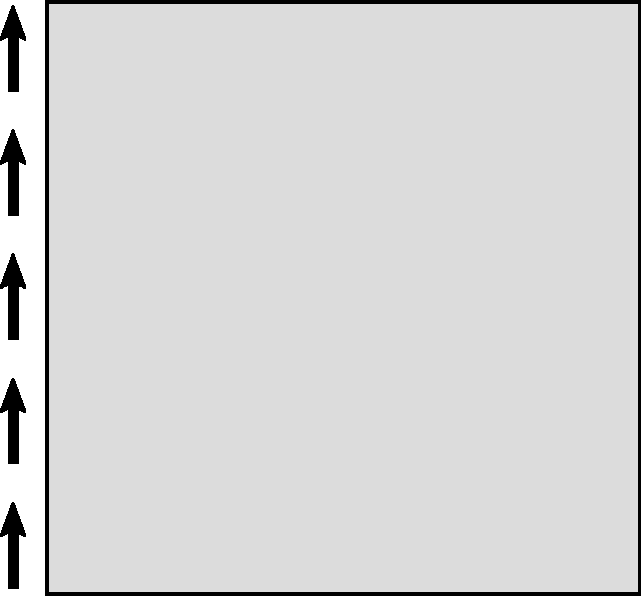
\includegraphics[height=0.3\textheight]{driven_cavity}
  \qquad
  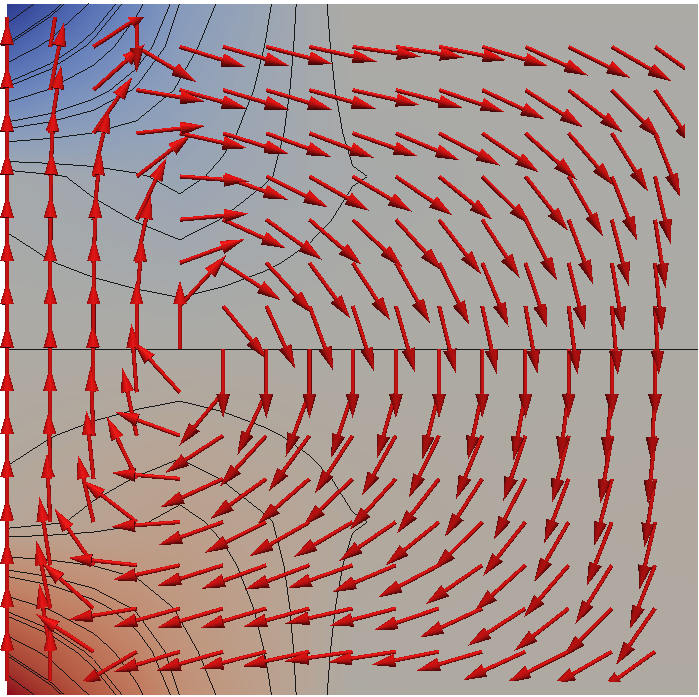
\includegraphics[height=0.3\textheight]{driven_cavity_result}
 \end{center}
 \caption{Driven cavity. Left: setting, right: simulation result.  The arrows show the {\em normalized} velocity.}
 \label{fig:driven_cavity}
\end{figure}

The Stokes equation models a viscous incompressible
fluid in a $d$-dimensional domain $\Omega$.  There are two unknowns in this problem: a stationary
fluid velocity field $\mathbf{u} : \Omega \to \R^d$, and the fluid pressure $p : \Omega \to \R$.
Together, they have to solve the boundary value problem
\begin{alignat*}{2}
 -\Delta \mathbf{u} - \nabla p & = 0  & \qquad & \text{in $\Omega$} \\
 \div \mathbf{u} & = 0                &        & \text{in $\Omega$} \\
                    \mathbf{u} & = \mathbf{u}_D  &        & \text{on $\partial \Omega$},
\end{alignat*}
where we have omitted the physical parameters.  The boundary value problem only determines the
pressure $p$ up to a constant function.  The pressure is therefore usually normalized such
that $\int_\Omega p\,dx = 0$.

Due to the constraint $\div \mathbf{u} = 0$, the corresponding weak form of the equation is a saddle-point problem.
Introduce the spaces
\begin{align*}
 \mathbf{H}^1_D(\Omega)
      & \colonequals
      \big\{ \mathbf{v} \in \mathbf{H}^1(\Omega) \; :\; \operatorname{tr}{\mathbf{v}} = \mathbf{u}_D \big\}, \\
 L_{2,0}(\Omega) & \colonequals  \Big\{ q \in L_2(\Omega) \; :\; \int_\Omega q\,dx = 0 \Big\},
\end{align*}
and the bilinear forms
\begin{equation*}
 a(\mathbf{u},\mathbf{v}) \colonequals \int_\Omega \nabla \mathbf{u} \nabla \mathbf{v} \,dx,
 \qquad \text{and} \qquad
 b(\mathbf{v},q) \colonequals \int_\Omega \div \mathbf{v} \cdot q \,dx.
\end{equation*}
Then the weak form of the Stokes equation is: Find $(\mathbf{u},p) \in \mathbf{H}_D^1(\Omega) \times L_{2,0}(\Omega)$ such that
\begin{alignat*}{2}
 a(\mathbf{u},\mathbf{v}) + b(\mathbf{v},p) & = 0 & \qquad & \text{for all $\mathbf{v} \in \mathbf{H}_0^1(\Omega)$} \\
 b(\mathbf{u},q)\qquad\qquad & = 0       &        & \text{for all $q \in L_{2,0}(\Omega)$}.
\end{alignat*}
If $\mathbf{u}_D$ is sufficiently smooth, this variational problem has a unique solution.
The Taylor--Hood element is the standard way to discretize this saddle point problem~\cite{braess:2013}.

\subsection{The driven-cavity benchmark}

For our example we choose to simulate a two-dimensional driven cavity.  This is a standard benchmark
for the Stokes problem in the literature.  Let $\Omega$ be the unit square $[0,1]^2$, and set the Dirichlet
boundary conditions for the velocity $\mathbf{u}$ to
\begin{equation*}
 \mathbf{u}(x)
 =
 \begin{cases}
  (0,1) & \text{if $x \in \{0\} \times [0,1]$} \\
  (0,0) & \text{elsewhere on $\partial \Omega$}.
 \end{cases}
\end{equation*}
The interpretation of this is a fluid container that is closed on all but one side.  While the fluid remains
motionless on the closed sides, an external agent drives a constant upward motion on the left vertical side.
The domain and boundary conditions are depicted in Figure~\ref{fig:driven_cavity}, left.
The corresponding solution is shown on the right side of the same figure.  The velocity forms a vortex,
while the pressure forms extrema in the two left corners.

In the following discussion we always use the letter $d$ to denote the space dimension, even though it is
known to be $d=2$ for our specific example.  This is to avoid confusion, because the number~2 also
appears a few times because we have two types of unknowns.

\subsection{Discretization}

\begin{figure}
  \begin{center}
   \begin{overpic}[width=0.5\textwidth]{taylor_hood_tree}
    \put(5,5){$P_2$}
    \put(30,5){$P_2$}
    \put(55,5){$P_2$}
    \put(87,31){$P_1$}
    \put(5,30){$V_\text{v}$}
    \put(5,57){$B_\text{TH}$}
    \put(30.7,32){$\otimes$}
    \put(61.6,58){$\otimes$}
   \end{overpic}

  \end{center}
  \caption{Taylor--Hood basis $P_2 \otimes P_2 \otimes P_2 \otimes P_1$ in a tree representation}
    \label{fig:taylor_hood_basis_tree}
\end{figure}

We discretize the domain using a structured axis-aligned grid with $4 \times 4$ uniform quadrilateral elements.
On this grid, we use the Taylor--Hood element to discretize the weak saddle-point problem.  The nodal basis
of the Taylor--Hood element has a natural tree structure as shown in Figure~\ref{fig:taylor_hood_basis_tree}.
On each element, the \dunemodule{dune-functions} implementation provides a local numbering of all shape functions
on this element.  This numbering uses a simple integer as index type, and is used to address the entries of the
element stiffness matrix.

\begin{table}
 \begin{center}
 \begin{tabular}{c|c}
 basis function & multi-index \\
 \hline \\
  $b_{x,0}$  & $(0,0)$ \\
  $b_{y,0}$  & $(0,1)$ \\
  $b_{z,0}$  & $(0,2)$ \\
  $b_{x,1}$  & $(0,3)$ \\
  $b_{y,1}$  & $(0,4)$ \\
  $b_{z,1}$  & $(0,5)$ \\
  $b_{x,2}$  & $(0,6)$ \\
  $b_{y,2}$  & $(0,7)$ \\
  $b_{z,2}$  & $(0,8)$ \\
    \vdots   & \vdots  \\
  $p_0$      & $(1,0)$ \\
  $p_1$      & $(1,1)$ \\
  $p_2$      & $(1,2)$ \\
    \vdots   & \vdots
 \end{tabular}
 \end{center}
 \caption{Multi-index for the Taylor--Hood basis with interleaved ordering of the velocity basis functions}
 \label{tbl:th_multiindices_interleaved}
\end{table}

Each global basis function additionally gets a global index, used to address the entries of the global stiffness
matrix.  In principle, \dunemodule{dune-functions} provides several types of orderings and multi-indices here.
The one that is used in the code example is given  in Table~\ref{tbl:th_multiindices_interleaved}: Each global
index is a pair $(a,b)$, where $a \in \{0,1\}$ switches between velocity and pressure basis functions,
and $b \in \mathbb{N}$ selects a particular basis function in either the set of velocity basis functions
or the set of pressure basis functions.


\subsection{Implementation}

This chapter discusses an example implementation of the Stokes problem, using only \dunemodule{dune-functions}
and no higher-level modules.  The example is contained in a single file, which comes as part of the \dunemodule{dune-functions}
source tree, in \file{dune-functions/examples/stokes-taylorhood.cc}.  If you read this document in electronic form,
the file can also be accessed by clicking on the icon in the margin.%
%
\marginpar{\attachfile[author=The dune-functions team,
                       color = 1 0 0,
                       mimetype=text/plain,
                       description=Complete source code of the Stokes/Taylor-Hood example]
                       {../../examples/stokes-taylorhood.cc}}

\subsubsection{The \texorpdfstring{\cpp{main}}{main} method}

We begin discussing the example code by describing its \cpp{main} method.  This method begins by setting up MPI and the grid.
We pick \cpp{YaspGrid} for the structured $4 \times 4$ quadrilateral grid.  Note that there is the line
%
\lstinputlisting[linerange={using_namespace_dune_begin-using_namespace_dune_end},
                 numbers=left]{../../examples/stokes-taylorhood.cc}
%
at the top of the file, so this namespace is imported completely.  Additionally, everything in the \dunemodule{dune-functions}
module is in the namespace \cpp{Functions}.  This namespace is not imported; instead, the prefix \cpp{Functions::} is always
given explicitly.


%
\lstinputlisting[linerange={main_begin-grid_setup_end},
                 numbers=left]{../../examples/stokes-taylorhood.cc}
%
The \cpp{gridView} object is the flat finite element grid that we will use for
the computation.
On this grid view, we then set up the function space basis for the Taylor--Hood element.  This is as simple as
%
\lstinputlisting[linerange={function_space_basis_begin-function_space_basis_end},
                 numbers=left]{../../examples/stokes-taylorhood.cc}
%
For each element, the \cpp{taylorHoodBasis} object will give us the tree of shape functions, and the corresponding local and global numberings.

Before being able to assemble the stiffness matrix of the Stokes system we need to pick suitable data structures
for the linear algebra.
The implementation of the Taylor--Hood basis selected in Line~\ref{li:stokes_taylorhood_select_taylorhoodbasis} orders the
velocity degrees of freedom before the pressure degrees of freedom.  Further, the velocity
components are interleaved.  The indexing scheme results from grouping degrees of freedom at the
tree root.  The resulting multi-indices all have length~2, and are given in Table~\ref{tbl:th_multiindices_interleaved}.
Consequently, the appropriate vector type is a pair of scalar vectors, one for the velocity and one for the pressure
degrees of freedom.  Analogously, the matrix must consist of $2 \times 2$ large sparse scalar matrices.
The following code sets up vector and matrix types for this, using the nesting machinery from \dunemodule{dune-istl}.
%
\lstinputlisting[linerange={linear_algebra_setup_begin-linear_algebra_setup_end},
                 numbers=left]{../../examples/stokes-taylorhood.cc}
%
Other index types are possible and possibly desirable here.  These would correspond to other vector and
matrix data types.

Now that we have chosen the C++ types for the matrix and vector data structures we can actually assemble the system.
Assembling the right-hand-side vector \cpp{rhs} is easy, because, apart from the Dirichlet boundary data (which we
will insert later), all its entries are zero.  An all-zero vector of the correct type and size is set up by the
following lines
%
\lstinputlisting[linerange={rhs_assembly_begin-rhs_assembly_end},
                 numbers=left]{../../examples/stokes-taylorhood.cc}
%
The \cpp{HierarchicVectorView} is a device that offers easier handling of arbitrarily nested vector data types.
In particular, it offers convenient resizing of an entire hierarchy of nested vectors.
The \cpp{taylorHoodBasis} object informs about the sizes of the corresponding finite element basis subtrees,
and Line~\ref{li:stokes_taylorhood_set_rhs_to_zero} fills the entire vector with zeros.

To obtain the stiffness matrix we first create an empty matrix object of the correct type.  The actual assembly
is factored out into a separate method.
%
\lstinputlisting[linerange={matrix_assembly_begin-matrix_assembly_end},
                 numbers=left]{../../examples/stokes-taylorhood.cc}
%
As the matrix assembly is the central part of this example we explain it in detail below, after having covered the \cpp{main} method.

Suppose now that we have the correct stiffness matrix assembled in the object \cpp{stiffnessMatrix}.  We still need
to modify the linear system to include the Dirichlet information.
In a first step we need to determine all degrees of freedom with Dirichlet data.  These are all the velocity degrees of freedom
on the domain boundary.  We could do this by using the \cpp{LocalKey} object of each basis function
to single out all those that are assigned to a boundary entity.  However, on a simple domain as the unit square
used here it is easier to use a geometric criterion.  We first define a predicate that returns \cpp{true}
if a given global coordinate \cpp{x} is on the domain boundary:
%
\lstinputlisting[linerange={boundary_predicate_begin-boundary_predicate_end},
                 numbers=left]{../../examples/stokes-taylorhood.cc}
%
The we interpolate this boolean-valued function in the space spanned by the velocity basis functions.
%
\lstinputlisting[linerange={interpolate_boundary_predicate_begin-interpolate_boundary_predicate_end},
                 numbers=left]{../../examples/stokes-taylorhood.cc}
%
Observe how the \dunemodule{dune-functions} interface allows to interpolate C++11 lambdas, which makes the code
very short and readable.  The expression \cpp{TypeTree::hybridTreePath(_0,i)} selects the different coordinate
directions of the velocity basis from the tree representation given in Figure~\ref{fig:taylor_hood_basis_tree}.
As the bases for the velocity components are all the same, an ordinary integer \cpp{i} is sufficient to choose
one of them.  In contrast, the velocity and pressure bases are different C++ types, and a compile-time
construction is needed to choose between them.  The object \cpp{_0} is defined in
\file{dune/typetree/utility.hh} as (roughly)
\begin{lstlisting}[style=Interface]
std::integer_constant<std::size_t, 0> _0;
\end{lstlisting}
In the \cpp{TaylorHoodBasis} implementation, \cpp{_0} selects the velocity subtree and \cpp{_1} selects
the pressure subtree.

Finally, we define a function implementing the actual Dirichlet values function $\mathbf{u}_D$, and interpolate
that into the right-hand-side vector \cpp{rhs}.
%
\lstinputlisting[linerange={interpolate_dirichlet_values_begin-interpolate_dirichlet_values_end},
                 numbers=left]{../../examples/stokes-taylorhood.cc}
%
The expression \cpp{TypeTree::hybridTreePath(_0)} demands that only velocity degrees of freedom are
interpolated.  The \cpp{isBoundary} vector given as the last argument restricts the interpolation
to only the boundary degrees of freedom.

The stiffness matrix is modified in a more manual fashion.  For each Dirichlet degree of freedom we need to fill the corresponding matrix row
with zeros, and write a~1 on the diagonal.  As only velocity
degrees of freedom have Dirichlet values, we need to modify the two upper matrix blocks only.
%
\lstinputlisting[linerange={set_dirichlet_matrix_begin-set_dirichlet_matrix_end},
                 numbers=left]{../../examples/stokes-taylorhood.cc}
%
Finally, we can solve the linear system.  Efficiently solving the Stokes system is an art, which we do not want to
get into here.  Instead, we a GMRes solver, without any preconditioner at all.  This is known to converge,
albeit slowly.
\todo[inline]{Eigentlich peinlich.  Können wir nicht doch einen vernünftigen Löser nehmen?}
The advantage is that it can be written down in very few lines.
%
\lstinputlisting[linerange={stokes_solve_begin-stokes_solve_end},
                 numbers=left]{../../examples/stokes-taylorhood.cc}
%
Observe how the \cpp{RestartedGMResSolver} object is completely oblivious to the fact that the matrix
has a two-level nesting structure.  On the other hand, dedicated Stokes solvers usually operate
on some sort of Schur complement, and hence they need direct access
to the four submatrices.  This can be elegantly done using the nested matrix type
used for the stiffness matrix.

Once the iterative solver has terminated, we write the result to a VTK file.  For this, we write the resulting velocity as a vector field,
and the resulting pressure as a scalar field.  We subsample the grid twice, because the \cpp{VTKWriter}
class natively only displays piecewise linear functions.
%
\lstinputlisting[linerange={stokes_output_begin-stokes_output_end},
                 numbers=left]{../../examples/stokes-taylorhood.cc}
%
When run, this program produces a file called \file{function-stokes-result.vtu}.  The file can be opened in
\program{ParaView}, and the outcome looks like the image on the right in Figure~\ref{fig:driven_cavity}.

\subsubsection{The global assembler}

Now that we have covered the \cpp{main} method, we can turn to the assembler for the Stokes stiffness matrix.
As our main focus is the use of the \dunemodule{dune-functions} interfaces, the assembler
is the central part of our example.   We begin with the global assembler,
which is the routine \cpp{assembleStokesMatrix} called in Line~\ref{li:stokes_taylorhood_call_to_assemblestokesmatrix}
of the \cpp{main} method.
The global assembler sets up the matrix pattern, loops over all elements, and accumulates the element stiffness
matrices in the global matrix. The signature of the method is
%
\lstinputlisting[linerange={global_assembler_signature_begin-global_assembler_signature_end},
                 numbers=left]{../../examples/stokes-taylorhood.cc}
%
The only arguments it gets are the finite element basis and the matrix to fill.  Observe that the Taylor--Hood basis is not
hard-wired here, so we could call the method with a different basis.
However, not surprisingly the assembler for the Stokes problem makes relatively tight assumptions on the basis tree
structure, so relatively little practical freedom is possible here.  Ideally, a global assembler should be fully
generic, and all knowledge about the current spaces and differential operators should be confined to the local
assembler.  Real discretization frameworks like \dunemodule{dune-pdelab} do achieve this separation,
but for our example here we are less strict, to avoid technicalities.

The first few lines of the \cpp{assembleStokesMatrix} method set up the matrix occupation pattern, and initialize the matrix with zeros.
%
\lstinputlisting[linerange={setup_matrix_pattern_begin-setup_matrix_pattern_end},
                 numbers=left]{../../examples/stokes-taylorhood.cc}
%
The actual pattern assembly is implemented in a separate method \cpp{getOccupationPattern}.
It returns a $2 \times 2$ table of \cpp{MatrixIndexSet} objects.
\todo[inline]{Erklären?  Überspringen?  Anders implementieren?}
The four \cpp{BCRSMatrix} objects are initialized with these patterns in Line~\ref{li:stokes_taylorhood_setup_matrix_patterns}.
Line~\ref{li:stokes_taylorhood_set_matrix_to_zero}
fills the entire matrix with zeros.

Next comes the actual element loop.  We first request a \cpp{localView} object and a \cpp{localIndexSet} object
from the finite element basis:
%
\lstinputlisting[linerange={get_localview_begin-get_localview_end},
                 numbers=left]{../../examples/stokes-taylorhood.cc}
%
After that, we start the loop over the grid elements.  For each element, we bind the \cpp{localView} object
to the element and the \cpp{localIndexSet} object to
the \cpp{localView}.  From now on all enquiries to the local view and index set will implicitly refer to this element.
%
\lstinputlisting[linerange={element_loop_and_bind_begin-element_loop_and_bind_end},
                 numbers=left]{../../examples/stokes-taylorhood.cc}
%
We then create the element stiffness matrix, and call the separate method \cpp{getLocalMatrix} to fill.
By default, \dunemodule{dune-functions} supposes that the element stiffness matrix is dense and non-hierarchical,
and Line~\ref{li:stokes_taylorhood_select_element_matrix_type}
picks a suitable type for such a matrix.
%
\lstinputlisting[linerange={setup_element_stiffness_begin-setup_element_stiffness_end},
                 numbers=left]{../../examples/stokes-taylorhood.cc}
%
The \cpp{getLocalMatrix} method is discussed in detail below.
In addition to the \cpp{elementMatrix} object, it gets only the \cpp{localView} object.  This object contains
all necessary information.

Finally, we loop over the entries of the element stiffness matrix and add them onto the global matrix.
%
\lstinputlisting[linerange={accumulate_global_matrix_begin-accumulate_global_matrix_end},
                 numbers=left]{../../examples/stokes-taylorhood.cc}
%
The type returned in Lines~\ref{li:stokes_taylorhood_get_global_row_index} and~\ref{li:stokes_taylorhood_get_global_column_index}
for the global row and column indices is a multi-index.  It has length~2 for both velocity degrees of freedom and for
pressure degrees of freedom.  Observe how Line~\ref{li:stokes_taylorhood_scatter_matrix_indices} uses the length-2
multi-index to access the nested matrix type.  For vectors, this scattering of multi-indices is implemented
in general form in the \cpp{HierarchicVectorWrapper} class.

The preceding loops write in particular into the lower right matrix block, even though we know that for the Stokes
system this block contains only zeros.  A more optimized version of the code would leave out the lower right
submatrix altogether.

\subsubsection{The local assembler}

Finally, we investigate the method that assembles the element stiffness matrices.  Its signature is
%
\lstinputlisting[linerange={local_assembler_signature_begin-local_assembler_signature_end},
                 numbers=left]{../../examples/stokes-taylorhood.cc}
%
As you see, it only receives the local view of the Taylor--Hood basis, expected to be bound to an element,
and the empty matrix.
The first few lines of the method gather some information about the element the method is to work on.
In particular, from the \cpp{localView} object it extracts the element itself, and the element's dimension and
geometry
%
\lstinputlisting[linerange={local_assembler_get_element_information_begin-local_assembler_get_element_information_end},
                 numbers=left]{../../examples/stokes-taylorhood.cc}
%
Next, the element stiffness matrix is initialized.  The \cpp{localView} object knows the total number of
degrees of freedom of the element it is bound to, and since the matrix is scalar this is the correct
number of matrix rows and columns.
%
\lstinputlisting[linerange={initialize_element_matrix_begin-initialize_element_matrix_end},
                 numbers=left]{../../examples/stokes-taylorhood.cc}
%
Finally, we first ask for the set of velocity and pressure shape functions.
%
\lstinputlisting[linerange={get_local_fe_begin-get_local_fe_end},
                 numbers=left]{../../examples/stokes-taylorhood.cc}
%
The two objects are \cpp{LocalFiniteElement}s in the \dunemodule{dune-localfunctions} sense of the word.
In fact, they are objects of the
\cpp{LocalFiniteElementVirtualInterface} class.  The virtual interface of \dunemodule{dune-localfunctions} is used here
because the Taylor--Hood basis implementation accommodates grids with more than a single element type.

In Lines~\ref{li:stokes_taylorhood_get_velocity_lfe}--\ref{li:stokes_taylorhood_get_pressure_lfe} you see the tree structure of the Taylor--Hood basis in action again:
The expression
\begin{lstlisting}[style=Example]
localView.tree().child(_0,0)
\end{lstlisting}
returns the first child of the first child of the root, i.e., the basis for the $x_0$-component of the velocity field,
and
\begin{lstlisting}[style=Example]
localView.tree().child(_1)
\end{lstlisting}
is the basis for the pressure space.
As the root of the tree combines two different bases, we need to use the static identifiers \cpp{_0} and \cpp{_1}
from the \cpp{Dune::TypeTree::Indices} namespace to specify its children.  The inner node for the velocities
combines $d$ times the same basis, and hence the normal integer \cpp{0} can be used to address its first child.
Our implementation of the local Stokes assembler is actually ``cheating'', because it exploits the knowledge
that the same basis is used for all velocity components.  Therefore, only the first leaf of the velocity
subtree is acquired in Line~\ref{li:stokes_taylorhood_get_velocity_lfe}, and then used for all components.
Using separate local finite elements is wasteful because the same shape function values and gradients
would be computed multiple times.

Next, we construct a suitable quadrature rule and loop over the quadrature points.  The formula for the quadrature
order combines information about the element type, the shape functions, and the differential operator.
\todo[inline]{\cpp{QuadratureRuleKey} verwenden!}
%
\lstinputlisting[linerange={begin_quad_loop_begin-begin_quad_loop_end},
                 numbers=left]{../../examples/stokes-taylorhood.cc}
%
The quadrature loop starts like similar local assembler codes seen elsewhere.
First, we get the inverse transposed Jacobian
of the map from the reference element to the grid element, and the Jacobian determinant for the integral
transformation formula
%
\lstinputlisting[linerange={quad_loop_preamble_begin-quad_loop_preamble_end},
                 numbers=left]{../../examples/stokes-taylorhood.cc}
%
With these preparations done, we can assemble the first part of the stiffness matrix,  corresponding to the
velocity--velocity coupling.  For two $d$-valued velocity basis functions $\bm{\varphi}_i^k = \mathbf{e}_k \varphi_i$
and $\bm{\varphi}_j^l = \mathbf{e}_l \varphi_j$ we need to compute
\begin{equation*}
 a(\bm{\varphi}_i^k, \bm{\varphi}_j^l)
 =
 \int_\Omega \nabla \bm{\varphi}_i^k \nabla \bm{\varphi}_j^l \,dx
 =
 \delta_{kl} \int_\Omega \nabla \varphi_i \nabla \varphi_j \,dx,
\end{equation*}
where $\varphi_i$ and $\varphi_j$ are the corresponding scalar basis functions.
The code first computes the derivatives of the velocity
shape functions at the current quadrature point,
and then uses the matrix in \cpp{jacobian} to transform the shape functions gradients to
gradients of the actual basis functions defined on the grid element.
%
\lstinputlisting[linerange={velocity_gradients_begin-velocity_gradients_end},
                 numbers=left]{../../examples/stokes-taylorhood.cc}
%
Withe the velocity basis function gradients at hand we can assemble the velocity contribution
to the stiffness matrix.
%
\lstinputlisting[linerange={velocity_velocity_coupling_begin-velocity_velocity_coupling_end},
                 numbers=left]{../../examples/stokes-taylorhood.cc}
%
Noteworthy here are the Lines~\ref{li:stokes_taylorhood_compute_vv_element_matrix_row}--\ref{li:stokes_taylorhood_compute_vv_element_matrix_column} which,
for two given shape functions from the finite element basis tree, compute the flat lexicographic numbering
used to index the element stiffness matrix.  The expression \cpp{child(_0,k)} singles out the tree leaf
for the \cpp{k}-th component of the velocity basis.  The loop variables \cpp{i} and \cpp{j} run over
the shape functions in this set, and
\begin{lstlisting}[style=Example]
localView.tree().child(_0,k).localIndex(i);
\end{lstlisting}
returns the corresponding scalar index for this shape function in the set of {\em all} shape functions
of the Taylor--Hood basis on this element.  Line~\ref{li:stokes_taylorhood_update_vv_element_matrix} then updates the corresponding (scalar)
element matrix entry with the correctly weighted product the two gradients $\nabla \varphi_i$
and $\nabla \varphi_j$.

Once this part is understood, computing, the velocity--pressure coupling terms is easy.
For a given velocity shape function $\bm{\varphi}_i^k$ and pressure shape function $\theta_j$ we need
to compute
\begin{equation*}
 b(\bm{\varphi}_i^k,\theta_j)
 =
 \int_\Omega \operatorname{div} \bm{\varphi}_i^k \cdot \theta_j\,dx
 =
 \int_\Omega \sum_{l=1}^d \frac{\partial (\bm{\varphi}_i^k)_l}{\partial x_l} \cdot \theta_j\,dx
 =
 \int_\Omega \frac{\partial \varphi_i}{\partial x_k} \cdot \theta_j\,dx
 =
 \int_\Omega (\nabla \varphi_i)_k \cdot \theta_j\,dx.
\end{equation*}
As additional information we need the values of the pressure basis functions $\{\theta_j\}$ at the
current quadrature point.  These are evaluated by the following two lines:
%
\lstinputlisting[linerange={pressure_values_begin-pressure_values_end},
                 numbers=left]{../../examples/stokes-taylorhood.cc}
%
Then, the actual matrix assembly is
%
\lstinputlisting[linerange={velocity_pressure_coupling_begin-velocity_pressure_coupling_end},
                 numbers=left]{../../examples/stokes-taylorhood.cc}
%
Line~\ref{li:stokes_taylorhood_compute_vp_element_matrix_row} computes the flat lexicographic index of $\bm{\varphi}_i^k$,
and Line~\ref{li:stokes_taylorhood_compute_vp_element_matrix_column} computes the index for $\theta_j$ (remember that \cpp{_1} denotes
the pressure basis).  Finally, Lines~\ref{li:stokes_taylorhood_update_vp_element_matrix_a}--\ref{li:stokes_taylorhood_update_vp_element_matrix_b}
then add the resulting terms to the matrix.




\section{Implementor interface}
\label{sec:implementation_api}

\todosander{Ich bin nicht davon überzeugt dass wir dieses Kapitel im Paper haben wollen.
Zum einen sind die internen Interfaces ja doch immer noch nicht wirklich stabil, und
man sollte sie deshalb aus einem ``offiziellen'' Dokument raushalten.  Zweitens muss
ja auch jemand den Text schreiben, und ich selbst würde vermutlich auf das Kapitel
verzichten bevor ich mir die Zeit nehme um es zu schreiben.}

The user interface is what is exposed by an actual basis for use in
application code. Any basis satisfying this interface is a valid
global basis in the \dunemodule{dune-functions} sense.
The implementors interface describes the reusable part of
a basis which is given by a \emph{pre-basis} in the following.
This interface allows to embed the pre-basis into a function space
basis of a larger space. This can be used, e.g., to compose
ansatz bases for mixed formulations, multicomponent problems,
or coupled multi-physic problems.


\subsection{Implementor interface of a \cpp{PreBasis}}
\subsection{Implementor interface of a \cpp{NodeIndexSet}}




\bibliographystyle{plainnat}
\bibliography{dune-functions-manual}

\end{document}

